%8 pages
%%
%% This is file `sample-sigconf.tex',
%% generated with the docstrip utility.
%%
%% The original source files were:
%%
%% samples.dtx  (with options: `sigconf')
%% 
%% IMPORTANT NOTICE:
%% 
%% For the copyright see the source file.
%% 
%% Any modified versions of this file must be renamed
%% with new filenames distinct from sample-sigconf.tex.
%% 
%% For distribution of the original source see the terms
%% for copying and modification in the file samples.dtx.
%% 
%% This generated file may be distributed as long as the
%% original source files, as listed above, are part of the
%% same distribution. (The sources need not necessarily be
%% in the same archive or directory.)
%%
%% The first command in your LaTeX source must be the \documentclass command.
%\documentclass[sigconf,table,anonymous]{acmart}
\documentclass[10pt,sigconf]{acmart}

\usepackage{algpseudocode}
\usepackage{algorithm}
\usepackage{algorithmicx}
\usepackage{verbatim}
\usepackage{mathtools}
\usepackage{multirow}
\usepackage{subcaption}
\usepackage{colortbl}
\usepackage{balance}

\usepackage{dirtree}

\usepackage{tikz}
\usetikzlibrary{fit,automata,positioning}
\usetikzlibrary{decorations.pathmorphing}
\tikzset{snake it/.style={decorate, decoration=snake}}

\definecolor{lightgray}{gray}{0.9}


%\def\BibTeX{{\rm B\kern-.05em{\sc i\kern-.025em b}\kern-.08em
	%	T\kern-.1667em\lower.7ex\hbox{E}\kern-.125emX}}

\usepackage{booktabs} % For formal tables

\usepackage{kbordermatrix} % include package @ document preamble
\renewcommand{\kbldelim}{(} % change default array delimiters to parentheses
\renewcommand{\kbrdelim}{)}

\newlength\Origarrayrulewidth

% horizontal rule equivalent to \cline but with 2pt width
\newcommand{\Cline}[1]{%
	\noalign{\global\setlength\Origarrayrulewidth{\arrayrulewidth}}%
	\noalign{\global\setlength\arrayrulewidth{3pt}}\cline{#1}%
	\noalign{\global\setlength\arrayrulewidth{\Origarrayrulewidth}}%
}

% draw a vertical rule of width 2pt on both sides of a cell
\newcommand\Thickvrule[1]{%
	\multicolumn{1}{!{\vrule width 2pt}c!{\vrule width 2pt}}{#1}%
}

% draw a vertical rule of width 2pt on the left side of a cell
\newcommand\Thickvrulel[1]{%
	\multicolumn{1}{!{\vrule width 2pt}c}{#1}%
}

% draw a vertical rule of width 2pt on the right side of a cell
\newcommand\Thickvruler[1]{%
	\multicolumn{1}{c!{\vrule width 2pt}}{#1}%
}

\newcommand\mc{\multicolumn{1}{c}{\cellcolor{lightgray}\textbf{1}}}

%%
%% \BibTeX command to typeset BibTeX logo in the docs
\AtBeginDocument{%
	\providecommand\BibTeX{{%
			\normalfont B\kern-0.5em{\scshape i\kern-0.25em b}\kern-0.8em\TeX}}}

%% Rights management information.  This information is sent to you
%% when you complete the rights form.  These commands have SAMPLE
%% values in them; it is your responsibility as an author to replace
%% the commands and values with those provided to you when you
%% complete the rights form.
\setcopyright{acmcopyright}
\copyrightyear{2021}
\acmYear{2021}
\acmConference[SIGMOD'21]{}{}{}
\acmBooktitle{}
\acmPrice{15.00}
\acmDOI{}
\acmISBN{XXX-X-XXXXX-XXX-X}


%%
%% Submission ID.
%% Use this when submitting an article to a sponsored event. You'll
%% receive a unique submission ID from the organizers
%% of the event, and this ID should be used as the parameter to this command.
%%\acmSubmissionID{123-A56-BU3}

%%
%% The majority of ACM publications use numbered citations and
%% references.  The command \citestyle{authoryear} switches to the
%% "author year" style.
%%
%% If you are preparing content for an event
%% sponsored by ACM SIGGRAPH, you must use the "author year" style of
%% citations and references.
%% Uncommenting
%% the next command will enable that style.
%%\citestyle{acmauthoryear}

\newtheorem{mytheorem}{Theorem}

\newcommand{\ltz}{$< 1$}

\algtext*{EndWhile}% Remove "end while" text
\algtext*{EndIf}% Remove "end if" text
\algtext*{EndFor}% Remove "end for" text
\algtext*{EndFunction}% Remove "end function" text

%%
%% end of the preamble, start of the body of the document source.
\begin{document}
	
	%%
	%% The "title" command has an optional parameter,
	%% allowing the author to define a "short title" to be used in page headers.
	\title[]{One Algorithm to Evaluate Them All: Unified Linear Algebra Based Approach to Evaluate Both Regular and Context-Free Path Queries}
	
	%%
	%% The "author" command and its associated commands are used to define
	%% the authors and their affiliations.
	%% Of note is the shared affiliation of the first two authors, and the
	%% "authornote" and "authornotemark" commands
	%% used to denote shared contribution to the research.
	
	\author{Ekaterina Shemetova}
	\email{katyacyfra@gmail.com}
	\affiliation{
		\institution{Saint Petersburg Academic University}
		\streetaddress{ 8/3 Khlopin St.}
		\city{St. Petersburg}
		\country{Russia}
		\postcode{---}
	}

	\author{Rustam Azimov}
	\email{rustam.azimov19021995@gmail.com}
	\affiliation{
		\institution{Saint Petersburg State University}
		\streetaddress{7/9 Universitetskaya nab.}
		\city{St. Petersburg}
		\country{Russia}
		\postcode{199034}
	}

    \author{Egor Orachyov}
	\email{egororachyov@gmail.com}
	\affiliation{%
		\institution{Saint Petersburg State University}
		\streetaddress{7/9 Universitetskaya nab.}
		\city{St. Petersburg}
		\country{Russia}
		\postcode{199034}
	}
	
	
	\author{Ilya Epelbaum}
	\email{iliyepelbaun@gmail.com}
	\affiliation{%
		\institution{Saint Petersburg State University}
		\streetaddress{7/9 Universitetskaya nab.}
		\city{St. Petersburg}
		\country{Russia}
		\postcode{199034}
	}
	

	\affiliation{
		\institution{JetBrains Research}
		\streetaddress{Primorskiy prospekt 68-70, Building 1}
		\city{St. Petersburg}
		\country{Russia}
		\postcode{199034}
	}
	
	
	\author{Semyon Grigorev}
	\email{s.v.grigoriev@spbu.ru}
	\email{semyon.grigorev@jetbrains.com}
	\orcid{0000-0002-7966-0698}
	\affiliation{
		\institution{Saint Petersburg State University}
		\streetaddress{7/9 Universitetskaya nab.}
		\city{St. Petersburg}
		\country{Russia}
		\postcode{199034}
	}
	\affiliation{
		\institution{JetBrains Research}
		\streetaddress{Primorskiy prospekt 68-70, Building 1}
		\city{St. Petersburg}
		\country{Russia}
		\postcode{199034}
	}
	
	%%
	%% By default, the full list of authors will be used in the page
	%% headers. Often, this list is too long, and will overlap
	%% other information printed in the page headers. This command allows
	%% the author to define a more concise list
	%% of authors' names for this purpose.
	\renewcommand{\shortauthors}{Shemetova et al.}
	
	%
	% The abstract is a short summary of the work to be presented in the article.
	\begin{abstract}
	We propose a new algo for CFPQ! 
	Abstract is very abstract. Abstract is very abstract. Abstract is very abstract. Abstract is very abstract. 
	Abstract is very abstract. Abstract is very abstract. Abstract is very abstract. Abstract is very abstract. 
	Abstract is very abstract. Abstract is very abstract. Abstract is very abstract. Abstract is very abstract. 
	Abstract is very abstract. Abstract is very abstract. Abstract is very abstract. Abstract is very abstract. 
	Abstract is very abstract. Abstract is very abstract. Abstract is very abstract. Abstract is very abstract. 
	Abstract is very abstract. Abstract is very abstract. Abstract is very abstract. Abstract is very abstract. 
	Abstract is very abstract. Abstract is very abstract. Abstract is very abstract. Abstract is very abstract. 
	Abstract is very abstract. Abstract is very abstract. Abstract is very abstract. Abstract is very abstract. 
	\end{abstract}
	
	%
	% The code below is generated by the tool at http://dl.acm.org/ccs.cfm.
	% Please copy and paste the code instead of the example below.
	%
	\begin{CCSXML}
		<ccs2012>
		<concept>
			<concept_id>10002951.10002952.10003197.10010825</concept_id>
			<concept_desc>Information systems~Query languages for non-relational engines</concept_desc>
			<concept_significance>500</concept_significance>
		</concept>
		<concept>
			<concept_id>10003752.10003766.10003771</concept_id>
			<concept_desc>Theory of computation~Grammars and context-free languages</concept_desc>
			<concept_significance>500</concept_significance>
		</concept>
		<concept>
			<concept_id>10003752.10003766.10003776</concept_id>
			<concept_desc>Theory of computation~Regular languages</concept_desc>
			<concept_significance>500</concept_significance>
		</concept>
		<concept>
			<concept_id>10002950.10003624.10003633.10003640</concept_id>
			<concept_desc>Mathematics of computing~Paths and connectivity problems</concept_desc>
			<concept_significance>500</concept_significance>
		</concept>
		<concept>
<concept_id>10002950.10003624.10003633.10010917</concept_id>
<concept_desc>Mathematics of computing~Graph algorithms</concept_desc>
<concept_significance>300</concept_significance>
</concept>
<concept>
<concept_id>10002951.10002952.10002953.10010146</concept_id>
<concept_desc>Information systems~Graph-based database models</concept_desc>
<concept_significance>500</concept_significance>
</concept>
		</ccs2012>
	\end{CCSXML}
	
    \ccsdesc[500]{Information systems~Graph-based database models}
	\ccsdesc[500]{Information systems~Query languages for non-relational engines}
	\ccsdesc[500]{Theory of computation~Grammars and context-free languages}
	\ccsdesc[500]{Theory of computation~Regular languages}
    \ccsdesc[500]{Mathematics of computing~Paths and connectivity problems}
	\ccsdesc[300]{Mathematics of computing~Graph algorithms}

	%
	% Keywords. The author(s) should pick words that accurately describe the work being
	% presented. Separate the keywords with commas.
	\keywords{}
	
	%%
	%% This command processes the author and affiliation and title
	%% information and builds the first part of the formatted document.
	\maketitle

\section{Introduction}

Scalable high-performance graph analysis is an actual challenge.
There is a big number of ways to attack this challenge~\cite{Coimbra2021} and the first promising idea is to utilize general-purpose graphic processing units (GPGPU).
Such existing solutions, as CuSha~\cite{10.1145/2600212.2600227} and Gunrock~\cite{7967137} show that utilization of GPUs can improve the performance of graph analysis, moreover it is shown that solutions may be scaled to multi-GPU systems.
But low flexibility and high complexity of API are problems of these solutions.

The second promising thing which provides a user-friendly API for high-performance graph analysis algorithms creation is a GraphBLAS API~\cite{7761646} which provides linear algebra based building blocks to create graph analysis algorithms.
The idea of GraphBLAS is based on a well-known fact that linear algebra operations can be efficiently implemented on parallel hardware.
Along with that, a graph can be natively represented using matrices: adjacency matrix, incidence matrix, etc.
While reference CPU-based implementation of GraphBLAS, SuiteSparse:GraphBLAS~\cite{10.1145/3322125}, demonstrates good performance in real-world tasks, GPU-based implementation is challenging.

One of the challenges in this way is that real data are often sparse, thus underlying matrices and vectors are also sparse, and, as a result, classical dense data structures and respective algorithms are inefficient. 
So, it is necessary to use advanced data structures and procedures to implement sparse linear algebra, but the efficient implementation of them on GPU is hard due to the irregularity of workload and data access patterns.
Though such well-known libraries as cuSPARSE show that sparse linear algebra operations can be efficiently implemented for GPGPU, it is not so trivial to implement GraphBLAS on GPGPU. 
First of all, it requires \textit{generic} sparse linear algebra, thus it is impossible just to reuse existing libraries which are almost all specified for operations over floats.
The second problem is specific optimizations, such as masking fusion, which can not be natively implemented on top of existing kernels.
Nevertheless, there is a number of implementations of GraphBLAS on GPGPU, such as GraphBLAST~\cite{yang2019graphblast}, GBTL~\cite{7529957}, which show that GPGPUs utilization can improve the performance of GraphBLAS-based graph analysis solutions.
But these solutions are not portable because they are based on Nvidia Cuda stack.
Moreover, the scalability problem is not solved: all these solutions support only single-GPU, not multi-GPU computations.

To provide portable GPU implementation of GraphBLAS API we developed a \textit{SPLA} library\footnote{Source code available at: \url{https://github.com/JetBrains-Research/spla}}.
This library utilizes OpenCL for GPGPU computing to be portable across devices of different vendors.
Moreover, it is initially designed to utilize multiple GPGPUs to be scalable.
To sum up, the contribution of this work is the following.
\begin{itemize}
    \item Design of portable GPU GraphBLAS implementation proposed. The design involves the utilization of multiple GPUS. Additionally, the proposed design is aimed to simplify library tuning and wrappers for different high-level platforms and languages creation. 
    \item Subset of GraphBLAS API, including such operations as masking, matrix-matrix multiplication, matrix-matrix e-wise addition, is implemented. The current implementation is limited by COO and CSR matrix representation format and uses basic algorithms for some operations, but work in progress and more data formats will be supported and advanced algorithms will be implemented in the future.
    \item Preliminary evaluation on such algorithms as breadth-first search (BFS) and triangles counting (TC), and real-world graphs shows portability across different vendors and promising performance: for some problems Spla is comparable with GraphBLAST. Surprisingly, for some problems, the proposed solution on embedded Intel graphic card shows better performance than SuiteSparse:GraphBLAS on the respective CPU. At the same time, the evaluation shows that further optimization is required.
\end{itemize} 
\section{Preliminaries}

In this section we introduce common definitions in graph theory and formal language theory which will be used in this paper. 
Also, we provide brief description of Azimov's algorithm which is used as a base of our solution.

\subsection{Graphs}

In this work we use edge-labelled digraph as a data model and define it as follows.
\begin{definition} \emph{Labeled directed graph} is a triple $D = (V,E,\sigma)$, where
\begin{itemize}
    \item $V$ is a set of vertices
    \item $E$ is a set of edges
    \item $\sigma \subseteq \Sigma$ is a set of labels, and a set of edges $E\subseteq V\times \sigma \times V$
\end{itemize}
\end{definition}

An example of the graph is presented in figure~\ref{fig:example_input_graph}.

\begin{figure}[h]
    \centering        
    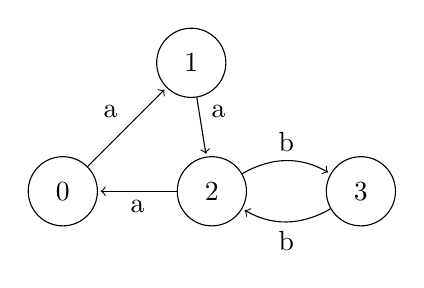
\begin{tikzpicture}[shorten >=1pt,auto]
       \node[state] (q_0)                      {$0$};
       \node[state] (q_1) [above right=of q_0] {$1$};
       \node[state] (q_2) [right=of q_0]       {$2$};
       \node[state] (q_3) [right=of q_2]       {$3$};
        \path[->]
        (q_0) edge  node {a} (q_1)
        (q_1) edge  node {a} (q_2)
        (q_2) edge  node {a} (q_0)
        (q_2) edge[bend left, above]  node {b} (q_3)
        (q_3) edge[bend left, below]  node {b} (q_2);
    \end{tikzpicture}
    \caption{The example of input graph $\mathcal{G}$}
    \label{fig:example_input_graph}
\end{figure}

We use adjacency matrix decomposed to a set of a boolean matrix as a representation of the graph.
\begin{definition}
An adjacency matrix $M$ of the graph $\mathcal{G}=$ is a square $|V|\times|V|$ matrix, such that $M[i,j] = \{l \mid e = (i,l,j) \in E\}$.
\end{definition}

Adjacency matrix $M$ of the graph $\mathcal{G}$ is

$$
    M =
    \begin{pmatrix}
    . & \{a\} & . & .     \\
    . & . & \{a\} & .     \\
    \{a\} & . & . & \{b\} \\
    . & . & \{b\} & .
    \end{pmatrix}.
$$

\begin{definition}

Boolean decomposition of adjacency matrix $M$ of graph $\mathcal{G}=$ is set of Boolean matrix $$\mathcal{M} = \{M^l \mid l \in L, M^l[i,j]=1 \iff l \in M[i,j]\}.$$

\end{definition}

Matrix $M$ can be represented as a set of two Boolean matrices $M^a$ and $M^b$ where
\begin{align}
M^{a} =
\begin{pmatrix}
    . & 1 & . & .   \\
    . & . & 1 & .   \\
    1 & . & . & .   \\
    . & . & . & .  
\end{pmatrix}, 
M^{b} =
\begin{pmatrix}      
    . & . & . & .   \\
    . & . & . & .   \\
    . & . & . & 1   \\
    . & . & 1 & . 
\end{pmatrix} \label{eq:boolean_decomposition_of_graph}
\end{align}
\subsection{Languages}

\begin{definition}\emph{Context-free grammar} is a 4-tuple $G=(N, \Sigma, R, S)$, where 
\begin{itemize}
    \item $N$ is a set of nonterminals
    \item $\Sigma$ is a set of terminals
    \item $R$ is a finite set of productions of the followings form: $A \to \alpha, ~A \in N,~ \alpha \in (N \cup \Sigma)^*$
    \item $S$ - a starting nonterminal
\end{itemize}
\end{definition}

\begin{definition} \emph{Context-free language} is a language generated by a context-free grammar:
\begin{align*}
     L(G) = \{w \in \Sigma^* \mid S \Rightarrow^* w \} 
\end{align*}
Where $S \Rightarrow^* w$  denotes that a string $w$ can be generated from a starting non-terminal $S$ using some sequence of production rules from $P$.
\end{definition}

\begin{definition} Context-free grammar $G = (N, \Sigma, R, S)$ is said to be in \emph{Chomsky normal form} if all productions in $R$ are of the form:
    \begin{itemize}
        \item $A \rightarrow BC,~A,~B,~C \in N$
        \item  $A \rightarrow a,~A \in N,~a \in \Sigma$
        \item $S \rightarrow \varepsilon,~\varepsilon$ is an empty string
    \end{itemize}
\end{definition}
Note that every context-free grammar can be transformed into an equivalent one in Chomsky Normal Form. 
\begin{definition} Context-free grammar $G = (N, \Sigma, P, S)$ is said to be in \emph{Weak Chomsky normal form} if all productions in $P$ are of the form:
    \begin{itemize}
        \item $A \rightarrow BC,~A,~B,~C \in N$
        \item  $A \rightarrow a,~A \in N,~a \in \Sigma$
        \item $A \rightarrow \varepsilon,~A \in N$
    \end{itemize}
\end{definition}
In other words, weak Chomsky normal form differs from Chomsky normal Form in the followings:
\begin{itemize}
    \item $\varepsilon$ can be derived from any non-terminal
    \item $S$ can be at a right part of productions
\end{itemize}
    
    
For example, let's consider the following context-free grammar, which generates the language $L(G) = \{A^nB^n, n \in \mathbb{N}\}$:
$G=(N, \Sigma, P, S), ~N=\{S\},~\Sigma=\{A,B\}$ and productions: 
\begin{align*}
S \rightarrow AB \\
S \rightarrow ASB\\
S \rightarrow \varepsilon
\end{align*}
After transformation to Chomsky Normal Form the resulting grammar:
\begin{align*}
S \rightarrow AB \\
S \rightarrow AC \\
C \rightarrow SB \\
S \rightarrow \varepsilon
\end{align*}

This productions itself are the grammar that has the same result as original grammar.

We use a context-free grammar in the weak Chomsky Normal Form without a starting non-terminal, which will be specified in the path queries for the graph. It should be noted that we omit the rules of the form $A \rightarrow \varepsilon$ for the reason that they correspond to trivial paths, which are more convenient to consider separately.

\begin{definition}\emph{Context-free relation} is a relation $R_A \subseteq V \times V$ for graph $G = (V, E)$, context-free grammar $G = (N,~\Sigma,~P)$ and fixed non-terminal $A$:
\begin{align*}
     R_A = \{(n, m) \mid \exists n \pi m~(l(\pi) \in L(G_A))\}
\end{align*}
\end{definition}

 Now, the definition for \emph{multiple-source (single-source) context-free path querying problem} can be formulated in the introduced notation as follows. For the given graph $G = (V, E)$, context-free grammar $G=(N, \Sigma, P)$ and set of source vertices $Src$ we need to find all context-free relations $R_A$ for any $A \in Src$. 
 
\subsection{Matrix-Based Algorithm}
Let $D = (V, E)$ be the input graph and $G = (N, \Sigma, P)$ be the input grammar. For the context-free path query evaluation, we need to provide context-free relations \mbox{$R_A \subseteq V \times V$} for every \mbox{$A \in N$}.
The matrix-based algorithm for CFPQ can be expressed in terms of operations over Boolean matrices (see listing~\ref{alg:algo0}) which is an advantage for implementation.
{\footnotesize
\begin{algorithm}
\begin{algorithmic}[1]
\caption{Context-free path querying algorithm}
\label{alg:algo0}
\Function{evalCFPQ}{$D=(V,E), G=(N,\Sigma,P)$}
    \State{$n \gets$ |V|}
    \State{$T \gets \{T^{A_i} \mid A_i \in N, T^{A_i}$ is a matrix $n \times n$, $T^{A_i}_{k,l} \gets$ \texttt{false}\} }
    \ForAll{$(i,x,j) \in E$, $A_k \mid A_k \to x \in P$}
        %\Comment{Matrices initialization}
        %\For{$A_k \mid A_k \to x \in P$}
          {$T^{A_k}_{i,j} \gets \texttt{true}$}
        %\EndFor
    \EndFor
    \ForAll{$A_k \mid A_k \to \varepsilon \in P$}
        \ForAll{$i \in \{0,\ldots ,n-1\}$}
            {$T^{A_k}_{i,i} \gets \texttt{true}$}
        \EndFor
    \EndFor

    \While{any matrix in $T$ is changing}
        %\Comment{Transitive c	losure calculation}
        \For{$A_i \to A_j A_k \in P$}
          { $T^{A_i} \gets T^{A_i} + (T^{A_j} \times T^{A_k})$ } 
        \EndFor
    \EndWhile
\State \Return $T$
\EndFunction
\end{algorithmic}
\end{algorithm}
}

This CFPQ algorithm allows efficiently apply GPGPU techniques, but it solves all-pairs problem and takes unreasonable amount of memory in scenarios in which we want to find paths from a relatively small set of vertices, since it calculates a lot of redundant information.  
\section{Context-free path querying by Kronecker product}

The algorithm consists of two parts: the firsy one is a index creation and the second one is a paths extraction (if required).

\subsection{Index Creation Algorithm}

The \textit{index creation} algorithm outputs the final adjacency matrix $\mathcal{M}_2$
for the input graph with all vertices pairs, which are reachable through some nonterminal 
in the input grammar $G$, and the index matrix $\mathcal{C}_3$, which allows to extract
paths in the \textit{path extraction} algorithm.

The algorithm is based on the generalization of the FSM intersection for an RSM, 
and the edge-labeled directed input graph. Since the RSM is composed as set of FSMs, 
it could be easily presented as adjacency matrix for some graph over labels set 
$\Sigma \cup S$. As shown in the Def.~\ref{def:bool:product} we can apply 
Kronecker product from Boolean matrices to \textit{intersect} the RSM and the 
input graph to some extent. But the RSM contains the nonterminal symbols from $N$ 
with additional \textit{recursive calls} logic, what requires \textit{transitive closure} 
step for such symbols extraction.

Applying the Kronecker product and transitive closure theory together, we get the idea 
of the algorithm: iterative Kronecker product evaluation for the RSM and the input 
graph, followed by transitive closure, nonterminal extraction and the update 
of the graph adjacency matrix.

% In this section, we introduce the algorithm for context-free path querying.
%The algorithm determines the existence of a path, which forms a sentence of the language defined by 
%the input RSM $R$, between each pair of vertices in the directed edge-labeled graph $\mathcal{G}$.
%The algorithm is based on the generalization of the FSM intersection for an RSM, 
%and an input graph. Since a graph can be interpreted as a FSM, in which 
%transitions correspond to the labeled edges between vertices of the graph, 
%and an RSM is composed of a set of FSMs, the intersection of such machines
%can be computed using the classical algorithm for FSM intersection, presented 
%in~\cite{automata:theory:10.5555/1177300}. 
%Such a way of generalization leads to zero-overhead algorithm for RPQ, contrary to other algorithms which require regular expression to context-free grammar transformation.

%The intersection can be computed as a Kronecker product of the corresponding 
%adjacency matrices for an RSM and a graph. Since we are only determining the
%reachability of vertices, it is enough to represent intersection result as 
%a Boolean matrix. It simplifies the algorithm implementation and allows 
%one to express it in terms of basic matrix operations.

%\subsubsection{Na{\"i}ve Version}
% Todo: reference to the algoritm description in the ADBIS paper 

\subsubsection{Boolean Matrices Based Version}
Listing~\ref{tensor:cfpq} shows main steps of the algorithm.
The algorithm accepts context-free grammar $G=(\Sigma,N,P$) and graph $\mathcal{G}=(V,E,L)$ as an input.
An RSM $R$ is created from the grammar $G$.
Note, that $R$ must have no $\varepsilon$-transitions.
$\mathcal{M}_1$ and $\mathcal{M}_2$ are the Boolean adjacency matrices for the machine 
$R$ and the graph $\mathcal{G}$ correspondingly.

Then for each vertex $i$ of the graph $\mathcal{G}$, the algorithm adds loops 
with non-terminals, which allows deriving $\varepsilon$-word.
Here the following rule is implied: each vertex of the graph is reachable 
by itself through an $\varepsilon$-transition. Since the machine $R$ does 
not have any $\varepsilon$-transitions, the $\varepsilon$-word could be 
derived only if a state $s$ in the box $B$ of the $R$ is both initial and final.
This data is queried by the $getNonterminals$ function for each state $s$.

The algorithm terminates when the matrix $\mathcal{M}_2$ stops changing.
Kronecker product of matrices $\mathcal{M}_1$ and $\mathcal{M}_2$ is evaluated
for each iteration.
The result is stored in $\mathcal{M}_3$ as a Boolean matrix. Since we are interested
only in the reachability of some vertices, there is no need to store a separate
Boolean matrix for each label from $\Sigma \cup N$. Therefore, we can 
collapse it into one Boolean matrix $\mathcal{M}'_3$, what is done in the next step.
These Boolean matrix could be interpreted as an adjacency matrix for some directed graph
without labels with the same set of the vertices, as in the graph formed by $\mathcal{M}_3$.
From that point of view the matrix $\mathcal{M}'_3$ has the following property 
from its definition: if some vertices connected by some path in the graph $\mathcal{G}(\mathcal{M}'_3)$ then these vertices are
connected by one or many paths in the graph $\mathcal{G}(\mathcal{M}_3)$.

For the given $\mathcal{M}'_3$ a $\mathcal{C}_3$ transitive closure matrix
is evaluated by the corresponding function call. 
Then the algorithm iterates over cells of the $\mathcal{C}_3$.
For the pair of indices $(i,j)$, it computes $s$ and $f$ --- 
the initial and final states in the recursive automata $R$ which relate 
to the concrete $\mathcal{C}_3[i,j]$ of the closure matrix.
If the given $s$ and $f$ belong to the same box $B$ of $R$, $s = q_B^0$, 
and $f \in F_B$, then $getNonterminals$ returns the respective nonterminal.
Then for each such nonterminal the respective matrix of the graph adjacency 
matrix $\mathcal{M}_2$ is updated and a new edge as a Boolean value in the 
appropriate cell is added.

The functions $getStates$ and $getCoordinates$ (see Listing~\ref{tensor:cfpq:help})
are used to map indices between Kronecker product arguments and the result matrix.
The Implementation appeals to the blocked structure of the matrix $\mathcal{C}_3$, 
where each block corresponds to some automata and graph edge.

The algorithm returns the computed path extraction index $\mathcal{C}_3$ and 
the updated matrix $\mathcal{M}_2$, which contains the initial 
graph $\mathcal{G}$ data as well as data for nonterminals from $N$.
If a cell $M_2^S[i,j]$ for any valid indices $i$ and $j$ and $S \in N$ 
contains $\{1\}$, then vertex $j$ is reachable from vertex $i$ in grammar $G$ for 
nonterminal $S$.

\begin{algorithm}[h]
\floatname{algorithm}{Listing}
\begin{algorithmic}[1]
\footnotesize
\caption{Kronecker product based CFPQ}
\label{tensor:cfpq}
\Function{contextFreePathQuerying}{G, $\mathcal{G}$}
    % Input data preparation
    \State{$R \gets$ Recursive automata for $G$}
    \State{$\mathcal{M}_1 \gets$ Boolean adjacency matrix for $R$}
    \State{$\mathcal{M}_2 \gets$ Boolean adjacency matrix for $\mathcal{G}$}
    \State{$\mathcal{C}_3 \gets$ The empty matrix}
    % Eps-transition handling for graph
    \For{$s \in 0..dim(\mathcal{M}_1)-1$}
        \For{$S \in \textit{getNonterminals}(R,s,s)$}
            \For{$i \in 0..dim(\mathcal{M}_2)-1$}
                % Or just $M_2^n[i,i] \gets M_2^n[i,i] \vee \{1\}$ ??? 
                \State{$M_2^S[i,i] \gets \{1\}$}
            \EndFor
        \EndFor
    \EndFor
    \While{Matrix $M_2$ is changing}
        % Kronecker product (i.e. partial intersection)
        \State{$\mathcal{M}_3 \gets \mathcal{M}_1 \otimes \mathcal{M}_2$}
        \Comment{Evaluate Kronecker product}
        % Collapse to single Boolean matrix
        \State{$\mathcal{M}'_3 \gets \bigvee_{M_3^a \in \mathcal{M}_3} M_3^a $}
        \Comment{Collapse to Boolean matrix}
        % Closure over Boolean matrix only
        \State{$\mathcal{C}_3 \gets \textit{transitiveClosure}(\mathcal{M}'_3)$}
        \State{$n \gets$ dim($M_3)$}
        \Comment{Matrix $\mathcal{M}_3$ size = $n \times n$}
        % Add non-terminals (possibly new)
        \For{$(i,j) \in [0..n-1] \times [0..n-1]$}
            \If{$\mathcal{C}_3[i,j]$}
                \State{$s, f \gets \textit{getStates}(C_3,i,j)$}
                \State{$x, y \gets \textit{getCoordinates}(C_3,i,j)$}
                \For{$S \in \textit{getNonterminals}(R,s,f)$}
                    \State{$M_2^S[x,y] \gets \{1\}$}
                \EndFor
            \EndIf
        \EndFor
    \EndWhile
\State \Return $\mathcal{M}_2,\mathcal{C}_3$
\EndFunction
\end{algorithmic}
\end{algorithm}

\begin{algorithm}[h]
\floatname{algorithm}{Listing}
\begin{algorithmic}[1]
\footnotesize
\caption{Help functions for Kronecker product based CFPQ}
\label{tensor:cfpq:help}
\Function{getStates}{$C, i, j$}
    \State{$r \gets dim(\mathcal{M}_1)$}
    \Comment{$mathcal{M}_1$ is Boolean adjacency matrix for $R$}
    \State \Return{$\left\lfloor{i / r}\right\rfloor, \left\lfloor{j / r}\right\rfloor$}
\EndFunction
\Function{getCoordinates}{$C, i, j$}
    \State{$n \gets dim(\mathcal{M}_2)$}
    \Comment{$\mathcal{M}_2$ is Boolean adjacency matrix for $\mathcal{G}$}
    \State \Return{$i \bmod n, j \bmod n$}
\EndFunction
\end{algorithmic}
\end{algorithm}

\begin{lemma}
    \label{lemma:algo:correctness}
    Let $\mathcal{G} = (V,E,L)$ be a graph and $G = \langle\Sigma, N, S, P\rangle$ be a grammar.
    Let $\mathcal{M}_{2,(k)}$ be an adjacency matrix $\mathcal{M}_2$ after the execution of some iteration $k \geq 0$ of the algorithm in Listing~\ref{tensor:cfpq}.
    Then for any valid indices $i, j$ and for each nonterminal $A \in N$ such that cell $M_{2,(k)}^A[i,j]$ contains $\{1\}$, the following statement holds: in the graph $\mathcal{G}$ $\exists i\pi j: A \xrightarrow{*} l(\pi)$.
\end{lemma}

\begin{proof}{(Proof by induction)}

    \textbf{Basis:} For $k = 0$ and the statement of the lemma holds, since
    $\mathcal{M}_{2,(0)} = \mathcal{M}_2$, where $\mathcal{M}_2$ is adjacency matrix of the graph $\mathcal{G}$. The nonterminals,
    which allow to derive $\varepsilon$-word, are also added at algorithm
    preprocessing step, since each vertex of the graph is reachable by itself 
    through an $\varepsilon$-transition.
    
    \textbf{Inductive step:} Assume that the statement of the lemma holds for any
    $k \leq (p - 1)$ and show that it also holds for $k = p$, where $p \geq 1$.
    
    For the algorithm iteration $p$ the Kronecker product $\mathcal{M}_3, \mathcal{M}'_3$ and transitive
    closure $\mathcal{C}_3$ are evaluated as described in the algorithm. By the properties
    of this operations, some edge $e = ((s,i),(f,j))$ exists in the directed
    graph, represented by adjacency matrix $\mathcal{C}_3$, if and only if $\exists s
    \pi ^{'} f$ in the RSM graph, represented by matrix $\mathcal{M}_1$, and 
    $\exists i \pi j$ in graph, represented by $\mathcal{M}_{2,(p-1)}$. Concatenated symbols 
    along the path $\pi^{'}$ form some derivation string v, composed from terminals
    and non-terminals, where $v \xrightarrow{*} l(\pi)$  by the inductive assumption.
    
    The new $\{1\}$ will be added to the cell $M_{2,(k)}^A[i,j]$ only if $s$ and $f$ 
    are initial and final states of some box of the RSM corresponding to 
    the non-terminal $A$. In this case, the grammar $G$ has the derivation rule
    $A \to v$, and by the inductive assumption $v \xrightarrow{*} l(\pi)$. Therefore, 
    $A \xrightarrow{*} l(\pi)$ and this completes the proof of the lemma.
    
\end{proof}

\begin{lemma}
    \label{lemma:algo:completeness}
    Let $\mathcal{G} = (V,E,L)$ be a graph and $G = \langle\Sigma, N, S, P\rangle$ be a grammar. 
    Let $\mathcal{M}_{2,(k)}$ be an adjacency matrix $\mathcal{M}_2$ after the execution of some iteration $k \geq 0$ of the algorithm in Listing~\ref{tensor:cfpq}.
    For any path $i \pi j$ in the graph $\mathcal{G}$ with word $l = l(\pi)$ if 
    exists the derivation tree of $l$ from the nonterminal $A$ of the grammar $G$ with the height $h \leq k+1$, then $M_{2,(k)}^A[i,j]$ contains $\{1\}$.

\end{lemma}

\begin{proof}{(Proof by induction)}

    \textbf{Basis:} Show that statement of the lemma holds for the $k = 0$. Matrix
    $\mathcal{M}_{2,(0)} = \mathcal{M}_2$ and edges of the graph $\mathcal{G}$ contains only labels from $L$. 
    Since the derivation tree of height $h = k + 1 = 1$ contains only one non-terminal 
    $A$ as a root and only symbols from $\Sigma \cup {\varepsilon}$ as leafs, 
    for all paths, which form a word with derivation tree of the height $h = 1$, 
    the corresponding nonterminals will be added to the $M_{2,(0)}^A[i,j]$ via preprocessing step. Thus, the lemma statement holds for the $k = 1$.

    \textbf{Inductive step:} Assume that the statement of the lemma hold for any
    $k \leq (p - 1)$ and show that it also holds for $k = p$, where $p \geq 2$.
    
    For the algorithm iteration $p$ the Kronecker product $\mathcal{M}_3, \mathcal{M}'_3$ and transitive
    closure $\mathcal{C}_3$ are evaluated as described in the algorithm. By the properties
    of this operations, some edge $e = ((s,i),(f,j))$ exists in the directed
    graph, represented by adjacency matrix $\mathcal{C}_3$, if and only if $\exists s
    \pi^{'} f$ in the RSM graph, represented by matrix $\mathcal{M}_1$, and 
    $\exists i \pi j$ in graph, represented by $\mathcal{M}_{2,(p-1)}$. 
    
    For any path $i \pi j$, such that exist derivation tree of height $h < p + 1$ 
    for the word $l(\pi)$ with root non-terminal $A$, the cell $M_{2,(p)}^A[i,j]$ contains $\{1\}$ by inductive assumption.
    
    Suppose, that exists derivation tree $T$ of height $h = p + 1$ with the root 
    non-terminal $A$ for the path $i \pi j$. The tree $T$ is formed as
    $A \to a_1 .. a_d, d \geq 1$ where $\forall x \in [1..d]$ $a_x$ is sub-tree of
    height $h_x \leq p$ for the sub-path $i_x \pi_x j_x$. 
    By inductive hypothesis, there exists path $\pi_x$ for each derivation sub-tree, 
    such that $i = i_1 \pi_1 i_2 .. i_{d} \pi_{d} j_{d} = j$ and concatenation 
    of these paths forms $i \pi j$, and the root nonterminals of 
    this sub-trees are included in the matrix $M_{2, (p - 1)}$. 
    
    Therefore, vertices $i_x ~\forall x \in [1..d]$ form path in the graph, 
    represented by matrix $\mathcal{M}_{2, (p-1)}$, with complete set of labels.
    Thus, new $\{1\}$ will be added to the cell $M_{2,(p)}^A[i,j]$ corresponding to the vertices $i$ and $j$ and nonterminal $A$. This completes the proof of the lemma.

\end{proof}

\begin{theorem}
    Let $\mathcal{G} = (V,E,L)$ be a graph and $G = \langle\Sigma, N, S, P\rangle$ be a grammar.
    Let $\mathcal{M}_{2}$ be a result adjacency matrix after the execution of the algorithm in Listing~\ref{tensor:cfpq}. Then for any valid indices $i, j$ and for each nonterminal $A \in N$ the following statement holds: the cell $M_{2,(k)}^A[i,j]$ contains $\{1\}$, if and only if there is a path $i\pi j$ in the graph $\mathcal{G}$ such that $ A \xrightarrow{*} l(\pi)$.
\end{theorem}{}
    
\begin{proof}
    
    This theorem is a consequence of the  
    Lemma~\ref{lemma:algo:correctness} and 
    Lemma~\ref{lemma:algo:completeness}.
    
\end{proof}{}

\begin{theorem}{}
    Let $\mathcal{G} = (V,E,L)$ be a graph and $G = \langle\Sigma, N, S, P\rangle$ be a grammar.
    The algorithm in Listing~\ref{tensor:cfpq} terminates in finite number of steps.
\end{theorem}

\begin{proof}
    
    The main \textit{while-loop} in the algorithm is executed while graph adjacency 
    matrix $\mathcal{M}_2$ is changing. Since the algorithm only adds the edges with 
    non-terminals from $N$, the maximum required number of iterations 
    is $|N| \times |V| \times |V|$, where each component has finite size. 
    This completes the proof of the theorem.
    
\end{proof}{}

% TODO: more accurate upper bound for the algorithm complexity 

\subsubsection{Application of Dynamic Transitive Closure}

In this subsection we show how to reduce the time complexity of the algorithm in Listing~\ref{tensor:cfpq} by avoiding redundant calculations. 


It is easy to see that the most time-consuming steps in this algorithm are the Kronecker product and transitive closure computations. Recall that the matrix $\mathcal{M}_2$ is always changed in incremental manner i. e. elements (edges) are added to $\mathcal{M}_2$ (and are never deleted from it) on each iteration of the algorithm in Listing~\ref{tensor:cfpq}. So one does not need to recompute the whole product or transitive closure if an appropriate date structure is maintained.


To deal with the Kronecker product computation, we use the left-distributivity of the Kronecker product. Let $\mathcal{A}_2$ be a matrix with newly added elements and $\mathcal{B}_2$ be a matrix with the all previously found elements, such that $\mathcal{M}_2 = \mathcal{A}_2 + \mathcal{B}_2$. Then by the left-distributivity of the Kronecker product we have $\mathcal{M}_1 \otimes \mathcal{M}_2 = \mathcal{M}_1 \otimes (\mathcal{A}_2 + \mathcal{B}_2) = \mathcal{M}_1\otimes \mathcal{A}_2 + \mathcal{M}_1 \otimes \mathcal{B}_2$. Notice that $\mathcal{M}_1 \otimes \mathcal{B}_2$ is known and is already in the matrix $\mathcal{M}_3$ and its transitive closure also is already in the matrix $\mathcal{C}_3$, because it was calculated on the previous iterations, so it is left to update some elements of $\mathcal{M}_3$ by computing $\mathcal{M}_1\otimes \mathcal{A}_2$, which can be done in $O(|\mathcal{A}_2||\mathcal{M}_1|)$ time, where $|\mathcal{A}|$ denotes the number of non-zero elements in a matrix $\mathcal{A}$.


The fast computation of transitive closure can be obtained by using incremental dynamic transitive closure technique. We use an approach by Ibaraki and Katoh~\cite{IBARAKI198395} to maintain dynamic transitive closure. The key idea of their algorithm is to recalculate reachability information only for those vertices, which become reachable after insertion of the certain edge (see Figure~\ref{edgeAdd} for details). The algorithm is presented in Listing~\ref{tensor:cfpq:dynamicTC} (we have slightly modified it to efficiently track new elements of the matrix $\mathcal{C}_3$). 

\begin{algorithm}[h]
\floatname{algorithm}{Listing}
\begin{algorithmic}[1]
\footnotesize
\caption{The dynamic transitive closure procedure}
\label{tensor:cfpq:dynamicTC}
\Function{add}{$C_3, i, j$}
       \State{$n \gets$ Number of rows in $C_3$}
        \State{$C_3' \gets$ Empty matrix of size $n \times n$}
        \For{$u \neq 0 \in$ checkCondition($C_3, i, j$)}
        \State{newReachablePairs($C_3, C_3', u, j$)}
        \EndFor
        \State \Return $C_3'$
\EndFunction
 \Function{checkCondition}{$C_3, i, j$}
        \State{$A \gets$ Empty array of size $n$}
        \For{$u \in 0...n \mid  u \neq j $}
    \Comment{$1 \wedge 1 = 0 \wedge 0 = 1 \wedge 0 = 0$; $0 \wedge 1 = 1$}
       \State{ $A[u] = C_3[u,j] \wedge C_3[u,i]$}
        \EndFor
\State \Return $A$
\EndFunction
 \Function{newReachablePairs}{$C_3, C_3', u, j$}
      \State{$C_3'[u,v] = C_3[u, v] \wedge C_3[j, v]$}
 \Comment{$1 \wedge 1 = 0 \wedge 0 = 1 \wedge 0 = 0$; $0 \wedge 1 = 1$}
\EndFunction
\end{algorithmic}
\end{algorithm}

\begin{figure}
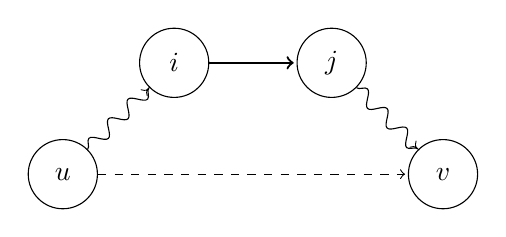
\begin{tikzpicture}[shorten >=1pt,node distance=2cm,on grid,auto] 
   \node[state] (q_0)   {$u$}; 
   \node[state] (q_1) [above right=of q_0] {$i$}; 
   \node[state] (q_2) [ right=of q_1] {$j$}; 
   \node[state] (q_3) [ below right=of q_2] {$v$}; 
    \path[->] 
    (q_0) edge[decorate, decoration={snake}]  node {} (q_1)
    (q_1) edge [thick]  node {} (q_2)
    (q_2) edge[decorate, decoration={snake}]  node {} (q_3)
    (q_0) edge [dashed]  node {} (q_3);        
\end{tikzpicture}

\caption{The vertex $j$ become reachable from the vertex $u$ after the addition of edge $(i, j)$. Then the vertex $v$ is reachable from $u$ after inserting the edge $(i, j)$ if $v$ is reachable from $j$.}
\label{edgeAdd}
\end{figure}

Final version of the modified algorithm from Listing~\ref{tensor:cfpq} is shown in Listing~\ref{tensor:cfpq:cubic}.

\begin{algorithm}[h]
\floatname{algorithm}{Listing}
\begin{algorithmic}[1]
\footnotesize
\caption{Kronecker product based CFPQ using dynamic transitive closure}
\label{tensor:cfpq:cubic}
\Function{contextFreePathQuerying}{G, $\mathcal{G}$}
    % Input data preparation
    \State{$R \gets$ Recursive automata for $G$}
    \State{$M_1 \gets$ Adjacency matrix for $R$}
    \State{$M_2 \gets$ Adjacency matrix for $\mathcal{G}$}
    \State{$A_2 \gets$ Adjacency matrix for $\mathcal{G}$}
    %\State{$M_3 \gets$ The empty matrix}
    \State{$C_3 \gets$ The empty matrix}
    % Eps-transition handling for graph
    \For{$s \in 0..dim(M_1)-1$}
        \For{$i \in 0..dim(M_2)-1$}
            \State{$M_2[i,i] \gets M_2[i,i] \cup \textit{getNonterminals}(R,s,s)$}
        \EndFor
    \EndFor
    \While{Matrix $M_2$ is changing}
       \State{$M_3' \gets  M_1 \otimes A_2$}
        \State{$A_2 \gets$ The empty matrix of size $n \times n$}
        %\Comment{Evaluate Kroncker product}
       \For{$M_3'[i,j] \mid M_3'[i,j] = 1$}
            \State{$C_3[i,j] \gets 1$}
             \State{$C_3' \gets  \bigcup_{(i,j)} \textit{add}(C_3, i, j)$}
             \Comment{Updating the transitive closure}
             \State{$C_3 \gets C_3 + C_3'$}
        \EndFor
        \State{$n \gets$ dim($M_3)$}
        %\Comment{Matrix $M_3$ size = $n \times n$}
        % Add non-terminals (possibly new)
        \For{$(i,j)\ |\ C_3'[i,j] \neq 0$}
                \State{$s, f \gets \textit{getStates}(C_3',i,j)$}
                \If{$\textit{getNonterminals}(R,s,f) \neq \emptyset$}
                    \State{$x, y \gets \textit{getCoordinates}(C_3',i,j)$}
                    \State{$M_2[x,y] \gets M_2[x,y] \cup \textit{getNonterminals}(R,s,f)$}
                     \State{$A_2[x,y] \gets A_2[x,y] \cup \textit{getNonterminals}(R,s,f)$}
                \EndIf
        \EndFor
    \EndWhile
\State \Return $\mathcal{M}_2, \mathcal{C}_3$
\EndFunction
\end{algorithmic}
\end{algorithm}
\begin{theorem}{}
    Let $\mathcal{G} = (V,E,L)$ be a graph and $G = \langle\Sigma, N, S, P\rangle$ be a grammar.
    The algorithm from Listing~\ref{tensor:cfpq:cubic} calculates a result matrices $\mathcal{M}_2$ and $\mathcal{C}_3$ in $O(n^3)$ time where $n = |V|$.
\end{theorem}

\begin{proof}
 Let $|\mathcal{A}|$ be a number of non-zero elements in a matrix $\mathcal{A}$. Consider the total time which is needed for computing the Kronecker products. The elements of the matrices $\mathcal{A}_2^{(i)}$ are pairwise distinct on every $i$-th iteration of the algorithm therefore we have 
 $$\sum\limits_i{T(\mathcal{M}_1 \otimes \mathcal{A}_2^{(i)})} = |\mathcal{M}_1| \otimes \sum\limits_i {|\mathcal{A}_2^{(i)}|} = |\mathcal{M}_1|O(n^2)$$
 operations in total. 


Now we derive the time complexity of maintainig the dynamic transitive closure. Notice that $C_3$ has size of $O(n^2)$ so no more than $O(n^2)$ edges will be added during all iterations of the Algorithm. The function $checkCondition$ from the Listing~\ref{tensor:cfpq:dynamicTC} takes $O(n)$ time for every inserted edge $(i, j)$. Thus we have $O(n^2n) = O(n^3)$ operations in total. The function $newReachablePairs$ requires $O(n)$ time for a given vertex $u$. This operation is performed for every pair $(j, v)$ of vertices such that a vertex $j$ became reachable from the vertex $u$. The vertex $j$ become reachable from the vertex $u$ (and accordingly the value of the matrix cell $C_3[u, j]$ becomes $1$ from $0$) only once during the entire computation, so the function $newReachablePairs$ will be executed at most $O(n^2)$ times for every $u$ and hence $O(n^3)$ times in total for all vertices. Therefore $O(n^3)$ operations are performed to maintain dynamic transitive closure during all iteration of the algorithm from Listing~\ref{tensor:cfpq:cubic}.


Notice that the matrix $\mathcal{C}_3'$ contains only new elements, therefore $\mathcal{C}_3$ can be updated directly using only $|\mathcal{C}_3'|$ operations and hence $O(n^2)$ operations in total. The same holds for cycle in line 18 of the algorithm from Listing~\ref{tensor:cfpq:cubic}, because operations are performed only for non-zero elements of the matrix $|\mathcal{C}_3'|$. Finally, we have that the time complexity of the algorithm is $O(n^2) + O(n^3) + O(n^2) + O(n^2) = O(n^3)$.
\end{proof}{}

\subsubsection{Speeding up by a factor of $\log n$}

In this subsection we use the Four Russians' trick to speed up the dynamic transitive closure algorithm from the Listing~\ref{tensor:cfpq:dynamicTC}.
\begin{theorem}{}
    The computation of transitive closure matrices can be done in $O(n^3/\log n)$ time when $n^2$ edges are added to the graph.
\end{theorem}
\begin{proof}
Consider the function $checkCondition$ from the Listing~\ref{tensor:cfpq:dynamicTC}. Its operations are equivalent to the element-wise (Hadamard) product of two vectors of size $n$, where multipication operation is denoted as $\wedge$ and has the following properties: $1 \wedge 1 = 0 \wedge 0 = 1 \wedge 0 = 0$ and $0 \wedge 1 = 1$. The first vector represents reachability of a given vertex $i$ from other vertices $\{u_1, u_2, ..., u_n\}$ of the graph and the second vector represents the same for a given vertex $j$. The function $newReachablePairs$ also can be reduced to the computation of the Hadamard product of two vectors of size $n$ for a given $u_k$. The first vector contains the information whether vertices  $\{v_1, v_2, ..., v_n\}$ of the graph are reachable from a given vertex $u_k$ and the second vector represents the same for a given vertex $j$. The element-wise product of two vectors can be calculated naively in time $O(n)$ which gives the $O(n^3)$ time for maintaining the transitive closure. Thus, the time complexity of the transitive closure can be reduced by speeding up element-wise product of two vectors of size $n$. 


To achive this goal, we use the Four Russians' trick. Split each vector into $n/\log n$ parts of size $\log n$. Create a table $S$ such that $S(a, b)$ = $a \wedge b$ where $a, b \ \in {\{0,1\}}^{\log n}$. This takes a time $O(n^2 \log n)$, since there are $2^{\log n} = n$ variants of Boolean vectors of size $\log n$ and hence $n^2$ pairs of vectors $(a, b)$ in total, and each component takes $O(\log n)$ time. With table $S$, we can calculate product of two parts of size $\log n$ in constant time. There are $n/\log n$ such parts, so the element-wise product of two vectors of size $n$ can be calculated in time $O(n/\log n)$ with $O(n^2 \log n)$ preprocessing. This gives us a dynamic transitive closure algorithm running in time $O(n^3/\log n)$: both of the functions $checkCondition$ and  $newReachablePairs$ are evaluated no more than $O(n^2)$ times during the whole computation, and each function calculates Hadamard product of two vectors in $O(n/\log n)$ time.
\end{proof} 
Notice that the maintaining of the dynamic transitive closure dominates the cost of the algorithm from Listing~\ref{tensor:cfpq:cubic}, therefore we immediately deduce the following.
\begin{corollary}{}
    Let $\mathcal{G} = (V,E,L)$ be a graph and $G = \langle\Sigma, N, S, P\rangle$ be a grammar.
    The result result matrices $\mathcal{M}_2$ and $\mathcal{C}_3$ can be calculated in $O(n^3/\log n)$ time.
\end{corollary}


Finally, we formulate the theorem which connects the time complexity of CFPQ and time complexity of specific incremental transitive closure of a directed graph.
\begin{theorem}{Subcubic incremental transitive closure leads to subcubic CFPQ.}
Suppose the incremental transitive closure problem where only insertion queries are allowed and the result of each insertion is a set of newly connected pairs. If one can solve this problem in $O(n^{3-\varepsilon})$ total time for $n^2$ insertions, then one can solve CFPQ in $O(n^{3-\varepsilon})$, where $n$ is a number of vertices in the graph in both cases. 
\end{theorem}
\subsection{Paths Extraction Algorithm}
After the index has been created, one can enumerate all paths between specified vertices.
The index stores information about all reachable pairs for all nonterminals.
Thus, the most natural way to use this index is to query paths between the specified vertices derivable from the specified nonterminal.
\begin{algorithm}[h]
\floatname{algorithm}{Listing}
\begin{algorithmic}[1]
\footnotesize
\caption{Paths extraction algorithm}
\label{tensor:pathsExtraction}
\State{$C_3 \gets $ result of index creation algorithm: final transitive closure}
\State{$\mathcal{M}_1 \gets $  the set of adjacency matrices of the input RSM}
\State{$\mathcal{M}_2 \gets $ the set of adjacency matrices of the final graph}

\Function{getPaths}{$v_s, v_f, N$}
    \State{$q_N^0 \gets$ Start state of automata for $N$}
    \State{$F_N \gets$ Final states of automata for $N$}
    \State{$res \gets \bigcup\limits_{f \in F_N} \Call{getPathsInner}{(q_N,v_s),(f,v_f)}$}
\State \Return $res$
\EndFunction

% DONE: fixed vertices notation (s,v)
% note: the first index in the pair is the state of the RSM
% note: the second index in the pair is the vertex of the graph

\Function{getSubpaths}{$(s_i,v_i), (s_j,v_j), (s_k,v_k)$}
    %\State{$v_i \gets \Call{getGraphV}{i}$}
    %\State{$v_k \gets \Call{getGraphV}{k}$}
    %\State{$v_j \gets \Call{getGraphV}{j}$}

    %\State{$s_i \gets \Call{getRsmState}{i}$}
    %\State{$s_k \gets \Call{getRsmState}{k}$}
    %\State{$s_j \gets \Call{getRsmState}{j}$}

  \State{\begin{minipage}[t]{0.2\textwidth}
           \vspace{-13pt}
           \begin{align*}
              l \gets & \{(v_i,t,v_k) \mid M_2^t[s_i, s_k] \wedge M_1^t[v_i, v_k]\}\\
                & \cup \ \bigcup_{\{N \mid M_2^N[s_i, s_k]\}}\Call{getPaths}{v_i, v_k, N} \\
                & \cup \ \Call{getPathsInner}{(s_i,v_i), (s_k,v_k)}
           \end{align*}
           \end{minipage}
          }
    \State{\begin{minipage}[t]{0.2\textwidth}
           \vspace{-13pt}
           \begin{align*}
              r \gets & \{(v_k,t,v_j) \mid M_2^t[s_k, s_j] \wedge M_1^t[v_k, v_j] \}\\
                      & \cup \ \bigcup_{\{N \mid M_2^N[s_k, s_j] \}}\Call{getPaths}{v_k, v_j, N} \\
                      & \cup \ \Call{getPathsInner}{(s_k,v_k), (s_j,v_j)}
           \end{align*}
           \end{minipage}
          }
    \State \Return $l \cdot r$
\EndFunction

\Function{getPathsInner}{$(s_i,v_i), (s_j,v_j)$}
    \State{$parts \gets \{ (s_k,v_k) \mid C_3[(s_i,v_i),(s_k,v_k)] = 1 \wedge C_3[(s_k,v_k),(s_j,v_j)] = 1\}$}
    \State \Return $\bigcup_{(s_k,v_k) \in parts} \Call{getSubpaths}{(s_i,v_i), (s_j,v_j),(s_k,v_k)}$
\EndFunction
\end{algorithmic}
\end{algorithm}

To do so, we provide a function \textsc{getPaths}($v_s, v_f, N$), where $v_s$ is a start vertex of the graph, $v_f$ --- the final vertex, and $N$ is a nonterminal.
Implementation of this function is presented in Listing~\ref{tensor:pathsExtraction}.

Paths extraction is implemented as three mutually recursive functions.
The entry point is \textsc{getPaths}($v_s, v_f, N$).
This function returns a set of the paths between $v_s$ and $v_f$ such that the word formed by a path is derivable from the nonterminal $N$.

To compute such paths, it is necessary to compute paths from vertices of the form $(q_N^s,v_s)$ to vertices of the form $(q_N^f, v_f)$ in the result of transitive closure, where $q_N^s$ is an initial state of RSM for $N$ and $q_N^f$ is a final state.
The function \textsc{getPathsInner}$((s_i,v_i),(s_j,v_j))$ is used to do it.
This function finds all possible vertices $(s_k,v_k)$  which split a path from $(s_i,v_i)$ to $(s_j,v_j)$ into two subpaths.
After that, function \textsc{getSubpaths}$((s_i,v_i),(s_j,v_j),(s_k,v_k))$ computes the corresponding subpaths.
Each subpath may be at least a single edge.
If single-edge subpath is labeled by terminal then corresponding edge should be added to the result else (label is nonterminal) \textsc{getPaths} should be used to restore paths.
If subpath is longer then one edge, \textsc{getPaths} should be used to restore paths. 

It is assumed that the sets are computed lazily, so as to ensure termination in the case of an infinite number of paths.
We also do not check paths for duplication manually, since they are assumed to be represented as sets.
\subsection{An example}

In this section we introduce detailed example to demonstrate steps of the proposed algorithm.
Our example is based on the classical worst case scenario introduced by Jelle Hellings in~\cite{!!!}. 
Namely, let we have a graph $\mathcal{G}$ presented in figure~\ref{fig:example_input_graph} and the RSM $R$ presented in figure~\cite{!!!}.

First step we represent graph as a set of boolean matrices as presented in~\ref{eq:boolean_decomposition_of_graph}, and RSM as a set of boolean matrices, as presented in~\ref{!!!}. 
Note, that we should add new empty matrix $M_2^{S}$ to $M_2$. 
After that we should iteratively compute $M_1$ and $C$. 

\textbf{First iteration.} As far as $M_2^{S,0}$ is empty (no edges with lable $S$ in the input graph), then correspondent block od the Kronecker product will be empty.
{\tiny
    \renewcommand{\arraystretch}{0.5}
    \setlength\arraycolsep{0.1pt}
\begin{align*}
& M_3^1 = M_1^a \otimes M_2^{a,0} +  M_1^b \otimes M_2^{b,0} + M_1^S \otimes M_2^{S,0} = \\
& \kbordermatrix{
          & (0,0) & (0,1) & (0,2) & (0,3) & \vrule & (1,0) & (1,1) & (1,2) & (1,3) & \vrule &  (2,0) & (2,1) & (2,2) & (2,3) & \vrule &  (3,0) & (3,1) & (3,2) & (3,3) &\\ 
    (0,0) & . & . & . & . & \vrule & . & 1 & . & . & \vrule & . & . & . & . &  \vrule & . & . & . & . \\
    (0,1) & . & . & . & . & \vrule & . & . & 1 & . & \vrule & . & . & . & . &  \vrule & . & . & . & . \\
    (0,2) & . & . & . & . & \vrule & 1 & . & . & . & \vrule & . & . & . & . &  \vrule & . & . & . & . \\
    (0,3) & . & . & . & . & \vrule & . & . & . & . & \vrule & . & . & . & . &  \vrule & . & . & . & . \\
    \hline
    (1,0) & . & . & . & .  & \vrule & . & . & . & . & \vrule & . & . & . & . & \vrule & . & . & . & . \\
    (1,1) & . & . & . & .  & \vrule & . & . & . & . & \vrule & . & . & . & . & \vrule & . & . & . & . \\
    (1,2) & . & . & . & .  & \vrule & . & . & . & . & \vrule & . & . & . & . & \vrule & . & . & . & 1 \\
    (1,3) & . & . & . & .  & \vrule & . & . & . & . & \vrule & . & . & . & . & \vrule & . & . & 1 & . \\
    \hline
    (2,0) & . & . & . & .  & \vrule & . & . & . & . & \vrule & . & . & . & . & \vrule & . & . & . & . \\
    (2,1) & . & . & . & .  & \vrule & . & . & . & . & \vrule & . & . & . & . & \vrule & . & . & . & . \\
    (2,2) & . & . & . & .  & \vrule & . & . & . & . & \vrule & . & . & . & . & \vrule & . & . & . & 1 \\
    (2,3) & . & . & . & .  & \vrule & . & . & . & . & \vrule & . & . & . & . & \vrule & . & . & 1 & . \\
    \hline
    (2,0) & . & . & . & .  & \vrule & . & . & . & . & \vrule & . & . & . & . & \vrule & . & . & . & . \\
    (2,1) & . & . & . & .  & \vrule & . & . & . & . & \vrule & . & . & . & . & \vrule & . & . & . & . \\
    (2,2) & . & . & . & .  & \vrule & . & . & . & . & \vrule & . & . & . & . & \vrule & . & . & . & . \\
    (2,3) & . & . & . & .  & \vrule & . & . & . & . & \vrule & . & . & . & . & \vrule & . & . & . & . \\
}
\end{align*}
}

Transitive closure calculation introduces one new path of length 2 (respective cell is filled). 

{\tiny
    \renewcommand{\arraystretch}{0.5}
    \setlength\arraycolsep{0.1pt}
\begin{align*}
& C_3^1 = tc(M_3^1) = 
\\
& \kbordermatrix{
          & (0,0) & (0,1) & (0,2) & (0,3) & \vrule & (1,0) & (1,1) & (1,2) & (1,3) & \vrule &  (2,0) & (2,1) & (2,2) & (2,3) & \vrule &  (3,0) & (3,1) & (3,2) & (3,3) &\\ 
    (0,0) & . & . & . & . & \vrule & . & 1 & . & . & \vrule & . & . & . & . &  \vrule & . & . & . & . \\
    (0,1) & . & . & . & . & \vrule & . & . & 1 & . & \vrule & . & . & . & . &  \vrule & . & . & . & \mc \\
    (0,2) & . & . & . & . & \vrule & 1 & . & . & . & \vrule & . & . & . & . &  \vrule & . & . & . & . \\
    (0,3) & . & . & . & . & \vrule & . & . & . & . & \vrule & . & . & . & . &  \vrule & . & . & . & . \\
    \hline
    (1,0) & . & . & . & .  & \vrule & . & . & . & . & \vrule & . & . & . & . & \vrule & . & . & . & . \\
    (1,1) & . & . & . & .  & \vrule & . & . & . & . & \vrule & . & . & . & . & \vrule & . & . & . & . \\
    (1,2) & . & . & . & .  & \vrule & . & . & . & . & \vrule & . & . & . & . & \vrule & . & . & . & 1 \\
    (1,3) & . & . & . & .  & \vrule & . & . & . & . & \vrule & . & . & . & . & \vrule & . & . & 1 & . \\
    \hline
    (2,0) & . & . & . & .  & \vrule & . & . & . & . & \vrule & . & . & . & . & \vrule & . & . & . & . \\
    (2,1) & . & . & . & .  & \vrule & . & . & . & . & \vrule & . & . & . & . & \vrule & . & . & . & . \\
    (2,2) & . & . & . & .  & \vrule & . & . & . & . & \vrule & . & . & . & . & \vrule & . & . & . & 1 \\
    (2,3) & . & . & . & .  & \vrule & . & . & . & . & \vrule & . & . & . & . & \vrule & . & . & 1 & . \\
    \hline
    (2,0) & . & . & . & .  & \vrule & . & . & . & . & \vrule & . & . & . & . & \vrule & . & . & . & . \\
    (2,1) & . & . & . & .  & \vrule & . & . & . & . & \vrule & . & . & . & . & \vrule & . & . & . & . \\
    (2,2) & . & . & . & .  & \vrule & . & . & . & . & \vrule & . & . & . & . & \vrule & . & . & . & . \\
    (2,3) & . & . & . & .  & \vrule & . & . & . & . & \vrule & . & . & . & . & \vrule & . & . & . & . \\
}
\end{align*}
}


This path starts in the vertex $(0,1)$ and finishes in the vertex $(3,3)$. 
We can see, that 0 is a start state of RSM $R$ and 3 is a final state of RSM $R$. Thus we can conclude that there esists a path between vertices 1 and 3 such that respective word is acceptable by $R$.
As a result we can add the edge $(1,S,3)$ to the $\mathcal{G}$, namely we should update the matrix $M_2^S$. 

\textbf{Second iteration.} Modified input graph contains edge with lable $S$. From now !!!

{\tiny
    \renewcommand{\arraystretch}{0.5}
    \setlength\arraycolsep{0.1pt}
\begin{align*}
& M_3^2 = M_1^a \otimes M_2^{a,0} +  M_1^b \otimes M_2^{b,0} + M_1^S \otimes M_2^{S,1} = \\
& \kbordermatrix{
          & (0,0) & (0,1) & (0,2) & (0,3) & \vrule & (1,0) & (1,1) & (1,2) & (1,3) & \vrule &  (2,0) & (2,1) & (2,2) & (2,3) & \vrule &  (3,0) & (3,1) & (3,2) & (3,3) &\\ 
    (0,0) & . & . & . & . & \vrule & . & 1 & . & . & \vrule & . & . & . & . &  \vrule & . & . & . & . \\
    (0,1) & . & . & . & . & \vrule & . & . & 1 & . & \vrule & . & . & . & . &  \vrule & . & . & . & . \\
    (0,2) & . & . & . & . & \vrule & 1 & . & . & . & \vrule & . & . & . & . &  \vrule & . & . & . & . \\
    (0,3) & . & . & . & . & \vrule & . & . & . & . & \vrule & . & . & . & . &  \vrule & . & . & . & . \\
    \hline
    (1,0) & . & . & . & .  & \vrule & . & . & . & . & \vrule & . & . & . & . & \vrule & . & . & . & . \\
    (1,1) & . & . & . & .  & \vrule & . & . & . & . & \vrule & . & . & . &\mc& \vrule & . & . & . & . \\
    (1,2) & . & . & . & .  & \vrule & . & . & . & . & \vrule & . & . & . & . & \vrule & . & . & . & 1 \\
    (1,3) & . & . & . & .  & \vrule & . & . & . & . & \vrule & . & . & . & . & \vrule & . & . & 1 & . \\
    \hline
    (2,0) & . & . & . & .  & \vrule & . & . & . & . & \vrule & . & . & . & . & \vrule & . & . & . & . \\
    (2,1) & . & . & . & .  & \vrule & . & . & . & . & \vrule & . & . & . & . & \vrule & . & . & . & . \\
    (2,2) & . & . & . & .  & \vrule & . & . & . & . & \vrule & . & . & . & . & \vrule & . & . & . & 1 \\
    (2,3) & . & . & . & .  & \vrule & . & . & . & . & \vrule & . & . & . & . & \vrule & . & . & 1 & . \\
    \hline
    (2,0) & . & . & . & .  & \vrule & . & . & . & . & \vrule & . & . & . & . & \vrule & . & . & . & . \\
    (2,1) & . & . & . & .  & \vrule & . & . & . & . & \vrule & . & . & . & . & \vrule & . & . & . & . \\
    (2,2) & . & . & . & .  & \vrule & . & . & . & . & \vrule & . & . & . & . & \vrule & . & . & . & . \\
    (2,3) & . & . & . & .  & \vrule & . & . & . & . & \vrule & . & . & . & . & \vrule & . & . & . & . \\
} \\
& C_3^2 = tc(M_3^2) = 
\\
& \kbordermatrix{
          & (0,0) & (0,1) & (0,2) & (0,3) & \vrule & (1,0) & (1,1) & (1,2) & (1,3) & \vrule &  (2,0) & (2,1) & (2,2) & (2,3) & \vrule &  (3,0) & (3,1) & (3,2) & (3,3) &\\ 
    (0,0) & . & . & . & . & \vrule & . & 1 & . & . & \vrule & . & . & . &\mc&  \vrule & . & . &\mc& . \\
    (0,1) & . & . & . & . & \vrule & . & . & 1 & . & \vrule & . & . & . & . &  \vrule & . & . & . & 1 \\
    (0,2) & . & . & . & . & \vrule & 1 & . & . & . & \vrule & . & . & . & . &  \vrule & . & . & . & . \\
    (0,3) & . & . & . & . & \vrule & . & . & . & . & \vrule & . & . & . & . &  \vrule & . & . & . & . \\
    \hline
    (1,0) & . & . & . & .  & \vrule & . & . & . & . & \vrule & . & . & . & . & \vrule & . & . & . & . \\
    (1,1) & . & . & . & .  & \vrule & . & . & . & . & \vrule & . & . & . & 1 & \vrule & . & . &\mc& . \\
    (1,2) & . & . & . & .  & \vrule & . & . & . & . & \vrule & . & . & . & . & \vrule & . & . & . & 1 \\
    (1,3) & . & . & . & .  & \vrule & . & . & . & . & \vrule & . & . & . & . & \vrule & . & . & 1 & . \\
    \hline
    (2,0) & . & . & . & .  & \vrule & . & . & . & . & \vrule & . & . & . & . & \vrule & . & . & . & . \\
    (2,1) & . & . & . & .  & \vrule & . & . & . & . & \vrule & . & . & . & . & \vrule & . & . & . & . \\
    (2,2) & . & . & . & .  & \vrule & . & . & . & . & \vrule & . & . & . & . & \vrule & . & . & . & 1 \\
    (2,3) & . & . & . & .  & \vrule & . & . & . & . & \vrule & . & . & . & . & \vrule & . & . & 1 & . \\
    \hline
    (2,0) & . & . & . & .  & \vrule & . & . & . & . & \vrule & . & . & . & . & \vrule & . & . & . & . \\
    (2,1) & . & . & . & .  & \vrule & . & . & . & . & \vrule & . & . & . & . & \vrule & . & . & . & . \\
    (2,2) & . & . & . & .  & \vrule & . & . & . & . & \vrule & . & . & . & . & \vrule & . & . & . & . \\
    (2,3) & . & . & . & .  & \vrule & . & . & . & . & \vrule & . & . & . & . & \vrule & . & . & . & . \\
}
\end{align*}
}

\begin{comment}
{\tiny
    \renewcommand{\arraystretch}{0.5}
    \setlength\arraycolsep{0.1pt}
\begin{align*}
& C_3^3 = 
\\
& \kbordermatrix{
          & (0,0) & (0,1) & (0,2) & (0,3) & \vrule & (1,0) & (1,1) & (1,2) & (1,3) & \vrule &  (2,0) & (2,1) & (2,2) & (2,3) & \vrule &  (3,0) & (3,1) & (3,2) & (3,3) &\\ 
    (0,0) & . & . & . & . & \vrule & . & 1 & . & . & \vrule & . & . & . & 1 &  \vrule & . & . & 1 & . \\
    (0,1) & . & . & . & . & \vrule & . & . & 1 & . & \vrule & . & . & . & . &  \vrule & . & . & . & 1 \\
    (0,2) & . & . & . & . & \vrule & 1 & . & . & . & \vrule & . & . &\mc& . &  \vrule & . & . & . &\mc\\
    (0,3) & . & . & . & . & \vrule & . & . & . & . & \vrule & . & . & . & . &  \vrule & . & . & . & . \\
    \hline
    (1,0) & . & . & . & .  & \vrule & . & . & . & . & \vrule & . & . & 1 & . & \vrule & . & . & . &\mc\\
    (1,1) & . & . & . & .  & \vrule & . & . & . & . & \vrule & . & . & . & 1 & \vrule & . & . & 1 & . \\
    (1,2) & . & . & . & .  & \vrule & . & . & . & . & \vrule & . & . & . & . & \vrule & . & . & . & 1 \\
    (1,3) & . & . & . & .  & \vrule & . & . & . & . & \vrule & . & . & . & . & \vrule & . & . & 1 & . \\
    \hline
    (2,0) & . & . & . & .  & \vrule & . & . & . & . & \vrule & . & . & . & . & \vrule & . & . & . & . \\
    (2,1) & . & . & . & .  & \vrule & . & . & . & . & \vrule & . & . & . & . & \vrule & . & . & . & . \\
    (2,2) & . & . & . & .  & \vrule & . & . & . & . & \vrule & . & . & . & . & \vrule & . & . & . & 1 \\
    (2,3) & . & . & . & .  & \vrule & . & . & . & . & \vrule & . & . & . & . & \vrule & . & . & 1 & . \\
    \hline
    (2,0) & . & . & . & .  & \vrule & . & . & . & . & \vrule & . & . & . & . & \vrule & . & . & . & . \\
    (2,1) & . & . & . & .  & \vrule & . & . & . & . & \vrule & . & . & . & . & \vrule & . & . & . & . \\
    (2,2) & . & . & . & .  & \vrule & . & . & . & . & \vrule & . & . & . & . & \vrule & . & . & . & . \\
    (2,3) & . & . & . & .  & \vrule & . & . & . & . & \vrule & . & . & . & . & \vrule & . & . & . & . \\
}
\end{align*}
}

{\tiny
    \renewcommand{\arraystretch}{0.5}
    \setlength\arraycolsep{0.1pt}
\begin{align*}
& C_3^4 = 
\\
& \kbordermatrix{
          & (0,0) & (0,1) & (0,2) & (0,3) & \vrule & (1,0) & (1,1) & (1,2) & (1,3) & \vrule &  (2,0) & (2,1) & (2,2) & (2,3) & \vrule &  (3,0) & (3,1) & (3,2) & (3,3) &\\ 
    (0,0) & . & . & . & . & \vrule & . & 1 & . & . & \vrule & . & . & . & 1 &  \vrule & . & . & 1 & . \\
    (0,1) & . & . & . & . & \vrule & . & . & 1 & . & \vrule & . & . & . &\mc&  \vrule & . & . &\mc& 1 \\
    (0,2) & . & . & . & . & \vrule & 1 & . & . & . & \vrule & . & . & 1 & . &  \vrule & . & . & . & 1\\
    (0,3) & . & . & . & . & \vrule & . & . & . & . & \vrule & . & . & . & . &  \vrule & . & . & . & . \\
    \hline
    (1,0) & . & . & . & .  & \vrule & . & . & . & . & \vrule & . & . & 1 & . & \vrule & . & . & . & 1\\
    (1,1) & . & . & . & .  & \vrule & . & . & . & . & \vrule & . & . & . & 1 & \vrule & . & . & 1 & . \\
    (1,2) & . & . & . & .  & \vrule & . & . & . & . & \vrule & . & . & . & 1 & \vrule & . & . &\mc& 1 \\
    (1,3) & . & . & . & .  & \vrule & . & . & . & . & \vrule & . & . & . & . & \vrule & . & . & 1 & . \\
    \hline
    (2,0) & . & . & . & .  & \vrule & . & . & . & . & \vrule & . & . & . & . & \vrule & . & . & . & . \\
    (2,1) & . & . & . & .  & \vrule & . & . & . & . & \vrule & . & . & . & . & \vrule & . & . & . & . \\
    (2,2) & . & . & . & .  & \vrule & . & . & . & . & \vrule & . & . & . & . & \vrule & . & . & . & 1 \\
    (2,3) & . & . & . & .  & \vrule & . & . & . & . & \vrule & . & . & . & . & \vrule & . & . & 1 & . \\
    \hline
    (2,0) & . & . & . & .  & \vrule & . & . & . & . & \vrule & . & . & . & . & \vrule & . & . & . & . \\
    (2,1) & . & . & . & .  & \vrule & . & . & . & . & \vrule & . & . & . & . & \vrule & . & . & . & . \\
    (2,2) & . & . & . & .  & \vrule & . & . & . & . & \vrule & . & . & . & . & \vrule & . & . & . & . \\
    (2,3) & . & . & . & .  & \vrule & . & . & . & . & \vrule & . & . & . & . & \vrule & . & . & . & . \\
}
\end{align*}
}

{\tiny
    \renewcommand{\arraystretch}{0.5}
    \setlength\arraycolsep{0.1pt}
\begin{align*}
& C_3^5 = 
\\
& \kbordermatrix{
          & (0,0) & (0,1) & (0,2) & (0,3) & \vrule & (1,0) & (1,1) & (1,2) & (1,3) & \vrule &  (2,0) & (2,1) & (2,2) & (2,3) & \vrule &  (3,0) & (3,1) & (3,2) & (3,3) &\\ 
    (0,0) & . & . & . & . & \vrule & . & 1 & . & . & \vrule & . & . &\mc& 1 &  \vrule & . & . & 1 &\mc\\
    (0,1) & . & . & . & . & \vrule & . & . & 1 & . & \vrule & . & . & . & 1 &  \vrule & . & . & 1 & 1 \\
    (0,2) & . & . & . & . & \vrule & 1 & . & . & . & \vrule & . & . & 1 & . &  \vrule & . & . & . & 1 \\
    (0,3) & . & . & . & . & \vrule & . & . & . & . & \vrule & . & . & . & . &  \vrule & . & . & . & . \\
    \hline
    (1,0) & . & . & . & .  & \vrule & . & . & . & . & \vrule & . & . & 1 & . & \vrule & . & . & . & 1\\
    (1,1) & . & . & . & .  & \vrule & . & . & . & . & \vrule & . & . & 1 & 1 & \vrule & . & . & 1 &\mc\\
    (1,2) & . & . & . & .  & \vrule & . & . & . & . & \vrule & . & . & . & 1 & \vrule & . & . & 1 & 1 \\
    (1,3) & . & . & . & .  & \vrule & . & . & . & . & \vrule & . & . & . & . & \vrule & . & . & 1 & . \\
    \hline
    (2,0) & . & . & . & .  & \vrule & . & . & . & . & \vrule & . & . & . & . & \vrule & . & . & . & . \\
    (2,1) & . & . & . & .  & \vrule & . & . & . & . & \vrule & . & . & . & . & \vrule & . & . & . & . \\
    (2,2) & . & . & . & .  & \vrule & . & . & . & . & \vrule & . & . & . & . & \vrule & . & . & . & 1 \\
    (2,3) & . & . & . & .  & \vrule & . & . & . & . & \vrule & . & . & . & . & \vrule & . & . & 1 & . \\
    \hline
    (2,0) & . & . & . & .  & \vrule & . & . & . & . & \vrule & . & . & . & . & \vrule & . & . & . & . \\
    (2,1) & . & . & . & .  & \vrule & . & . & . & . & \vrule & . & . & . & . & \vrule & . & . & . & . \\
    (2,2) & . & . & . & .  & \vrule & . & . & . & . & \vrule & . & . & . & . & \vrule & . & . & . & . \\
    (2,3) & . & . & . & .  & \vrule & . & . & . & . & \vrule & . & . & . & . & \vrule & . & . & . & . \\
}
\end{align*}
}
\end{comment}

{\tiny
    \renewcommand{\arraystretch}{0.5}
    \setlength\arraycolsep{0.1pt}
\begin{align*}
& C_3^6 = 
\\
& \kbordermatrix{
          & 0_{(0,0)} & 1_{(0,1)} & (0,2) & (0,3) & \vrule & (1,0) & (1,1) & (1,2) & (1,3) & \vrule &  (2,0) & (2,1) & (2,2) & (2,3) & \vrule &  (3,0) & (3,1) & (3,2) & (3,3) &\\ 
    0:(0,0) & . & . & . & . & \vrule & . & 1 & . & . & \vrule & . & . & 1 & 1 &  \vrule & . & . & 1 & 1 \\
    1:(0,1) & . & . & . & . & \vrule & . & . & 1 & . & \vrule & . & . & . & 1 &  \vrule & . & . & 1 & 1 \\
    2:(0,2) & . & . & . & . & \vrule & 1 & . & . & . & \vrule & . & . & 1 &\mc&  \vrule & . & . &\mc& 1 \\
    3:(0,3) & . & . & . & . & \vrule & . & . & . & . & \vrule & . & . & . & . &  \vrule & . & . & . & . \\
    \hline
    4:(1,0) & . & . & . & .  & \vrule & . & . & . & . & \vrule & . & . & 1 & 1 & \vrule & . & . &\mc& 1\\
    5:(1,1) & . & . & . & .  & \vrule & . & . & . & . & \vrule & . & . & 1 & 1 & \vrule & . & . & 1 & 1 \\
    6:(1,2) & . & . & . & .  & \vrule & . & . & . & . & \vrule & . & . & . & 1 & \vrule & . & . & 1 & 1 \\
    7:(1,3) & . & . & . & .  & \vrule & . & . & . & . & \vrule & . & . & . & . & \vrule & . & . & 1 & . \\
    \hline
    8:(2,0) & . & . & . & .  & \vrule & . & . & . & . & \vrule & . & . & . & . & \vrule & . & . & . & . \\
    9:(2,1) & . & . & . & .  & \vrule & . & . & . & . & \vrule & . & . & . & . & \vrule & . & . & . & . \\
    10:(2,2) & . & . & . & .  & \vrule & . & . & . & . & \vrule & . & . & . & . & \vrule & . & . & . & 1 \\
    11:(2,3) & . & . & . & .  & \vrule & . & . & . & . & \vrule & . & . & . & . & \vrule & . & . & 1 & . \\
    \hline
    12:(2,0) & . & . & . & .  & \vrule & . & . & . & . & \vrule & . & . & . & . & \vrule & . & . & . & . \\
    13:(2,1) & . & . & . & .  & \vrule & . & . & . & . & \vrule & . & . & . & . & \vrule & . & . & . & . \\
    14:(2,2) & . & . & . & .  & \vrule & . & . & . & . & \vrule & . & . & . & . & \vrule & . & . & . & . \\
    15:(2,3) & . & . & . & .  & \vrule & . & . & . & . & \vrule & . & . & . & . & \vrule & . & . & . & . \\
}
\end{align*}
}

Result is presented in figure~\ref{fig:example_result}.
New edges is added to the original graph.

\begin{figure}[h]
    \centering         
    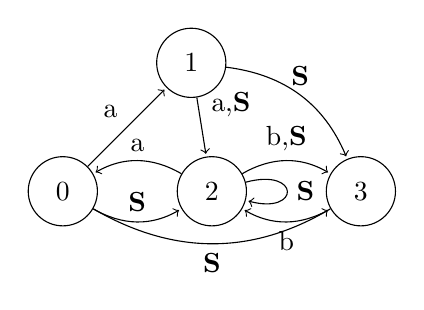
\begin{tikzpicture}[shorten >=1pt,auto]
    \node[state] (q_0)                      {$0$};
    \node[state] (q_1) [above right=of q_0] {$1$};
    \node[state] (q_2) [right=of q_0]       {$2$};
    \node[state] (q_3) [right=of q_2]       {$3$};
      \path[->]
        (q_0) edge node {a} (q_1)
        (q_1) edge node {a,\textbf{S}} (q_2)
        (q_2) edge[bend right, above]  node {a} (q_0)
        (q_2) edge[loop right]  node {\textbf{S}} (q_2)
        (q_1) edge[bend left, above]  node {\textbf{S}} (q_3)
        (q_0) edge[bend right, above]  node {\textbf{S}} (q_2)
        (q_2) edge[bend left, above]  node {b,\textbf{S}} (q_3)
        (q_0) edge[bend right, below]  node {\textbf{S}} (q_3)
        (q_3) edge[bend left, below]  node {b} (q_2);
    \end{tikzpicture}
    \caption{The result graph $\mathcal{G}$}
    \label{fig:example_result}    
\end{figure}


Index creation is finished. 
Onw can use it to unswer reachcbility queryes, but for some problems it is necessary to restore paths.
One can do it by using index created. 
Let for example we try to restore path from 2 to 2 derived from $S$.

To do it one should call \verb|getPaths(2, 2, s)|.
Partial trace of this call is presented below in figure~\ref{trc:exmaple}. 
First, we convert vertices from grap to indeces in matrix and call \verb|getPathsInner|.
Separation vertex \verb|pats={4}| and try to get patrs of paths going throw vertex with $id=4$.
\begin{figure}
\begin{minipage}[t]{0.48\textwidth}
{
\scriptsize
\setlength{\DTbaselineskip}{8pt}
\DTsetlength{0.2em}{0.5em}{0.2em}{0.4pt}{1.6pt}
\dirtree{%
.1 getPaths($2,2,S$).
.2 getPathsInner($2,14$).
.3 parts$=\{4\}$ parts = {4, 11} FIX IT!!!.
.3 getSubpaths($2,14,4$).
.4 l=$\{2 \xrightarrow{a} 0\}$.
.5 $\cdots$.
.6 getPathsInner($0,14$).
.7 parts = $\{5,11\}$.
.7 getSubpaths(0, 14, 5).
.8 $\cdots$.
.9 getPaths(1, 3, S).
.10 $\cdots$.
.11 getSubpaths(1,15,6).
.12 $l=\{ 1 \xrightarrow{a} 2 \}$.
.12 $r=\{ 2 \xrightarrow{b} 3 \}$.
.12 return $\{ 1\xrightarrow{a} 2 \xrightarrow{b} 3 \}$.
.7 getSubpaths(0, 14, 11).
.8 $\cdots$.
.9 getPaths(1, 3, S) // \begin{minipage}[t]{4cm}An alternative way to get paths from 1 to 3 which leads to infinite set of paths \end{minipage}.
.10 return $r_\infty^{1\leadsto 3}$ // \begin{minipage}[t]{4.5cm} An infinite set of path from 1 to 3 \end{minipage}.
.8 $\cdots$.
.7 return $\{0 \xrightarrow{a} 1 \xrightarrow{a} 2 \xrightarrow{b} 3 \xrightarrow{b} 2\} \cup (\{0 \xrightarrow{a} 1\} \cdot r_\infty^{1\leadsto 3} \cdot \{3 \xrightarrow{b} 2\})$ .
.2 return $\{2 \xrightarrow{a} 0 \xrightarrow{a} 1 \xrightarrow{a} 2 \xrightarrow{a} 0 \xrightarrow{a} 1 \xrightarrow{a} 2 \xrightarrow{b} 3 \xrightarrow{b} 2 \xrightarrow{b} 3 \xrightarrow{b} 2 \xrightarrow{b} 3 \xrightarrow{b} 2\} \cup (\{2 \xrightarrow{a}  0 \xrightarrow{a} 1 \xrightarrow{a} 2 \xrightarrow{a} 0 \xrightarrow{a} 1\} \cdot r_\infty^{1\leadsto 3} \cdot \{3 \xrightarrow{b} 2 \xrightarrow{b} 3 \xrightarrow{b} 2 \xrightarrow{b} 3 \xrightarrow{b} 2\})$.
}
}
\caption{Example of call stack trace}
\label{trc:exmaple}
\end{minipage}
\end{figure}


Expected path is returned, other paths calcualtion

Lazy evaluation is required.

The paths enumeration problem is actual here: ho can we enumerate paths with small delay.

\section{Implementation Details}

Currenly, our goal is to evaluate the applicability of the proposed algorithm, thus we implemented its naive version.
We compute the transitive closure from scratch on each iteration and do not use any incremental techniques.
In our implementation we use PyGraphBLAS\footnote{GitHub repository of PyGraphBLAS, a Python wrapper for GraphBLAS API: \url{https://github.com/michelp/pygraphblas}. Access date: 07.07.2020.} --- a Python wrapper for SuiteSparse library~\cite{10.1145/3322125}\footnote{Web page of SuiteSparse:GraphBLAS library: \url{http://faculty.cse.tamu.edu/davis/GraphBLAS.html}. Access date: 07.07.2020.}.
SuiteSparse is a C implementation of GraphBLAS~\cite{7761646} standard which introduces linear algebra building blocks for implementation of graph analysis algorithms.
Thus we provide a highly-optimized parallel CPU implementation of the naive version of the algorithm\footnote{Implementation of the described algorithm is published here: \url{anonimized/url/to/our/repo/with/sources}. Access date: 07.07.2020.}.%{https://github.com/JetBrains-Research/CFPQ_PyAlgo}. Access date: 07.07.2020.}.

At present, we do not integrate with a graph database and a graph query language.
We suppose that the input graph is stored in a file, while the query is expressed in terms of a context-free grammar and is also stored in file.
As it was shown in~\cite{10.1145/3398682.3399163}, it is possible to integrate SuiteSparse based implementation in the RedisGraph database.
Providing integration with a query language requires a lot of technical effort to extend the language.
There are existing proposals, for example to extend the Cypher language\footnote{Cypher language extension proposal which introduces a syntax to express context-free queries: \url{https://github.com/thobe/openCypher/blob/rpq/cip/1.accepted/CIP2017-02-06-Path-Patterns.adoc}. Access date: 07.07.2020.}.

Paths extraction is implemented in Python by using PyGraphBLAS.
Since lazy evaluation is not natural for Python, we cap the maximal number of paths to extract in the implementation.

\section{Evaluation}

This section describes the methodology and answers the following research questions.

\begin{enumerate}
    \item Does fusion via distillation give any benefits at the software and hardware levels?
    \item What are the properties of the generated hardware?
    \item Does the generated hardware outperform software implementations?
\end{enumerate}

\subsection{Methodology}

Our focus is on creating a basis for future research and experiments, thus we make our experiments as much reproducible as possible\footnote{\url{https://github.com/sedwards-lab/fhw/tree/sparse-linear-algebra-distillation/examples/QTreeBenchmarks/diploma/verilog-bool-no-nnz-inlined} (online; accessed:
2022-06-07) Here one could find all the results. For each benchmark all statistics are specified: matrix names, their sizes, collected metrics for both hardware and software benchmarks.}. We benchmarked the following list of chained functions. The choice is prompted by the current state of the distiller: at the moment, it does not successfully distill matrix multiplication. However, the functions are still practical enough, for example, chained addition could be seen in Luby's maximal independent set algorithm and clearly describe the applicability of the proposed approach.

\begin{itemize}
    \item \mintinline{Haskell}{mAdd (==False) (||) (mAdd (==False) (||) m1 m2) m3}
    \item \mintinline{Haskell}{mask (mAdd (== False) (||) m2 m3) (m1)}
    \item \mintinline{Haskell}{map (==Zero) (to_nat) (mAdd (==False) (||) m1 m2}
    \item \mintinline{Haskell}{map (==Zero) (to_nat) (kron (==False) (&&) m1 m2}
\end{itemize}

Above, \mintinline{Haskell}{Zero} and \texttt{to\_nat} are corresponding definitions for Peano arithmetics, since the \texttt{.pot} language does not have any primitives. For the same reason, we operated with boolean matrices. Such functions could be abstracted with free variables and then instantiated in the emitted Haskell code. However, to get maximum from distillation, we provided all the information about the functions. 

For these functions, we compared the execution time of distilled and not distilled hardware generated circuits, execution time of original and distilled Haskell code and reference \textit{Suite Sparse}\footnote{\url{https://github.com/DrTimothyAldenDavis/GraphBLAS} (online; accessed:
2022-06-07), Suite Sparse library sources.}\textsuperscript{,}\footnote{The library also uses different variations of coordinate formats (opaque to the user) and not a quadtree representation.} variants of these functions in C\texttt{++}. Note that SuiteSparse does not support recursive data types, thus only the first two function chains were implemented in SuiteSparse (since Peano number is essentially a linked list). We did not replace Peano numbers with integers, so our experiments could be interpreted easier. For hardware experiments we collected execution time and the number of memory writes and reads, to access how well fusion is performed. For software experiments we only measured the execution time. Also note that we measured only the time, required to execute the lines above, not including any IO, required to get and evaluate function arguments. But in hardware benchmarks we measured the time required to pass arguments into the circuit's memory, because such IO is inevitable. It is tricky to make such measures in Haskell due to laziness, thus the programs were compiled with \texttt{--fno-full-laziness} to turn off memoization. Also all the arguments were forced to normal form via \texttt{force} and \texttt{evaluate}. Haskell programs were compiled\footnote{GHC 8.10.4.} with \texttt{-O2 --fno-full-laziness} and Suite Sparse was compiled with default flags and linked as a shared library to C\texttt{++} code.

We took matrices from SuiteSparse matrix collection with sizes ranging from \texttt{64x64} to \texttt{512x512}. We limited ourselves with such sizes due to the fact that this is the maximum sizes that fit into \texttt{bram} with $2^{16}$ address space. Such number of \texttt{bram} blocks is available only on really expensive FPGA boards, thus in practice sizes would be smaller to achieve better utilization. Once again, it models the situation when data fits into the cache, since \texttt{bram} in our circuits will operate as a cache in real application.

\subsection{Experiments}

Table~\ref{tab:bench_results} shows the results of all execution time benchmarks. To evaluate execution time for hardware simulation, implementation stage was performed to assess the maximum frequency of FPGA device used for synthesis and implementation, and the number of execution cycles was multiplied by the number of nanoseconds a clock cycle takes. The frequencies were equal within the same benchamark set, i.e., frequency was not affected by distillation. We used \texttt{xcu250figd2104-2L} device\footnote{\url{https://www.xilinx.com/products/boards-and-kits/alveo/u250.html}  (online; accessed:
2022-06-07)} for synthesis and implementation stages. It is not really a casual and affordable chip, but it contains enough \texttt{bram} for our evaluation to see scalability. In the table a median across several benchmarks is shown. 

As it could be seen, distillation steadily increases performance: up to 2x speedup for hardware simulation and up to 3x for software benchmarks. The results are maintained within the borders of the corresponding confidence interval and the borders are not shown for brevity. Hardware speedup is lower due to the different execution semantics, dataflow is not reduction-based and distillation is a reduction-based transformation. Note that generated hardware appears to be less performant than both Haskell and C\texttt{++}, which a bit contradicts the results from~\cite{oldfhw}. For hardware benchmarks \texttt{time (IO)} shows the execution time including the time needed to transfer the data though the arguments, \texttt{time (no IO)} does not include it in its turn. It could be seen that not all the benchmarks are computationally extensive enough to cover memory transferring costs, but for more complex examples the ratio would be better. Since we basically transfer the matrices node by node from a file in the testbench, we have probably the lowest possible latency, and in practice it would be higher if reading from DDR, however the bandwidth could be increased. Noticeably, running times for \texttt{mMaskAdd} for C\texttt{++} and distilled Haskell are similar, which shows that fusion really provides some extra performance: SuiteSparse at the moment does not implement any fusion.

Table~\ref{tab:mem_results} summarizes the ratios between distilled and not distilled hardware circuits memory reads and writes. Since in general case distillation removes extra pattern matching, essentially it saves memory reads and writes. The eventual number of memory reads and writes is implementation dependent, thus the table shows what share of speedup is prompted by saving memory operations. Distillation successfully reduces the number of memory accesses, about 15\% on average. \texttt{mMapKron} has a bit higher ratio due to the fact that \texttt{Nat} numbers require additional memory accesses, since the type is recursive. It could also be seen that a major part of speedups is attributed to saved memory accesses. 

Finally, table~\ref{tab:resource_util} shows device resources utilization ratios between distilled and not distilled hardware circuits and frequencies. Columns are device primitives: registers, lookup tables, \texttt{bram} blocks or multiplexers. Utilization for both types of circuits is below 1\% of available resources on the device, except for the memory. Memory blocks utilization is about 30\% (since we choose larger \texttt{brams} to store larger matrices). Apart from that, distilled circuits could have both higher and lower utilization. Since the hardware generation is primarily syntax-directed it follows from the distilled program structure. For example, distillation might glue two recursive functions into one (in that case, memory utilization would be lower, because each cluster of mutually recursive functions possesses its own heap) or make more recursive functions than in the original program. The frequencies are the same, however, they possibly could be made better with more intelligent buffer allocation.

\subsection{Discussion}
Answering the research questions above.

\begin{enumerate}
    \item Fusion gives significant benefits, however at the hardware level the benefits are a bit smaller since hardware semantics is not reduction based. The benefits at the hardware level are mostly determined by the reduced number of memory accesses (each access takes 2 clock cycles). Notably, distilled Haskell implementation of \texttt{mMaskAdd} has similar performance with C\texttt{++}. 
    \item Device utilization is low, but such circuits could be copied on the same device to provide better utilization and higher parallelism. Resource utilization might be both better and worse after distillation, depending on the transformed program itself since translation is syntax-directed. Frequency could be increased by more intelligent buffering strategy.
    \item Although we use low-latency design with \texttt{bram}s that take 2 clock cycles per request and transfer matrices from files, which does not have any latency in simulation, we get slower execution time than Haskell and C\texttt{++} counterparts. It could be partly due to excessive buffering performed by FHW at the moment. Also there is no pipelining for recursive calls, i.e. only one set
of function argument tokens are allowed to enter a tail-recursive function call until a result is finally generated. Further CPS transformation hinders parallelization, which could be made more explicit with SSA. Some other optimizations exist that may significantly influence the performance. Also, since device utilization is about 1\%, such circuits could be copied on one device and provide more parallelism. A more detailed discussion could be found at~\cite{Edwards2019FHWP}.
\end{enumerate}

Distillation clearly showed its applicability to optimization of sparse linear algebra routines and notably it still could be combined with other techniques, like rewrite rules to achieve better results. High-level synthesis has a room for improvements by increasing pipelining, parallelism and frequency and the generated hardware could be improved from usability perspective: a support for arbitrary sized matrices is desirable. Thus we will focus on these directions. Probably a better solution would be to embed \texttt{.pot} language into e.g. Haskell to leverage its type system (to be able to use some rewrite rules as well), and add support for primitive types and parallel primitives to be able to conduct a more scalable comparison with SuiteSparse (since SuiteSparse is multithreaded). For such embedding different execution models could be implemented, including hardware synthesis, for which SSA form of GRIN looks promising, as well as extra optimizations shipped with GRIN. For hardware synthesis, an interesting direction is achieving predictable results in hardware from certain modifications in software. This property partly holds for the current approach, since the translation is syntax- directed. More information on this could be found at~\cite{predict}.

\pagebreak

\begin{table}[t]
\scriptsize
\centering
\caption*{mAddAdd}
\begin{tabular}{|c|c|c|c|c|c|c|c|c|c|} 
\hline
\rowcolor{LightBlue}
\multicolumn{3}{|c|}{Matrices dimensions} & Haskell & Haskell (distilled) & \multicolumn{2}{c|}{FHW} & \multicolumn{2}{c|}{FHW (distilled)} & {C\texttt{++}}\\
% \rowcolor{LightBlue}
\hline
m1 & m2 & m3 & time & time & time (no IO) & time (IO) & time (no IO) & time (IO) & time \\ 
\hline
64 & 64 & 64 & 29 us & 20 us & 76 us & 170 us & 64 us & 158 us & 14 us\\ 
128 & 128 & 128 & 94 & 79 & 146 & 476 & 134 & 469 & 30 \\
256 & 256 & 256 & 123 & 103 & 202 &  681 & 168 & 662 & 44\\
512 & 512 & 512 & 219 & 143 & 474 & 1192 & 375 & 1093 & 49\\
\hline
\end{tabular}

\caption*{mMaskAdd}
\begin{tabular}{|c|c|c|c|c|c|c|c|c|c|} 
\hline
\rowcolor{LightBlue}
\multicolumn{3}{|c|}{Matrices dimensions} & Haskell & Haskell (distilled) & \multicolumn{2}{c|}{FHW} & \multicolumn{2}{c|}{FHW (distilled)} & {C\texttt{++}}\\
% \rowcolor{LightBlue}
\hline
m1 & m2 & m3 & time & time & time (no IO) & time (IO) & time (no IO) & time (IO) & time \\ 
\hline
64 & 64 & 64 & 10 us & 7 us & 64 us & 133 us & 46 us & 111 us & 18 us\\ 
128 & 128 & 128 & 38 & 30 & 118 & 322 & 75 & 292 & 33 \\
256 & 256 & 256 & 48 & 42 & 168 &  498 & 104 & 456 & 46\\
512 & 512 & 512 & 126 & 76 & 400 & 762 & 300 & 729 & 65\\
\hline
\end{tabular}

\caption*{mMapAdd}
\begin{tabular}{|c|c|c|c|c|c|c|c|c|c|} 
\hline
\rowcolor{LightBlue}
\multicolumn{3}{|c|}{Matrices dimensions} & Haskell & Haskell (distilled) & \multicolumn{2}{c|}{FHW} & \multicolumn{2}{c|}{FHW (distilled)} & {C\texttt{++}}\\
% \rowcolor{LightBlue}
\hline
m1 & m2 & m3 & time & time & time (no IO) & time (IO) & time (no IO) & time (IO) & time \\ 
\hline
64 & 64 & --- & 45 us & 37 us & 189 us & 253 us & 137 us & 202 us & ---\\ 
128 & 128 & --- & 162 & 105 & 524 & 685 & 397 & 579 & --- \\
256 & 256 & --- & 312 & 216 & 1047 &  1360 & 680 & 986 & ---\\
512 & 512 & --- & 436 & 273 & 1346 & 1776 & 900 & 1330 & ---\\
\hline
\end{tabular}

\caption*{mMapKron}
\begin{tabular}{|c|c|c|c|c|c|c|c|c|c|} 
\hline
\rowcolor{LightBlue}
\multicolumn{3}{|c|}{Matrices dimensions} & Haskell & Haskell (distilled) & \multicolumn{2}{c|}{FHW} & \multicolumn{2}{c|}{FHW (distilled)} & {C\texttt{++}}\\
% \rowcolor{LightBlue}
\hline
m1 & m2 & m3 & time & time & time (no IO) & time (IO) & time (no IO) & time (IO) & time \\ 
\hline
2 & 64 & --- & 64 us & 36 us & 212 us & 242 us & 94 us & 125 us & ---\\ 
2 & 128 & --- & 137 & 68 & 434 & 502 & 199 & 266 & --- \\
2 & 256 & --- & 364 & 126 & 1004 &  1188 & 449 & 636 & ---\\
4 & 128 & --- & 302 & 94 & 694 & 763 & 330 & 401 & ---\\
\hline
\end{tabular}



\caption{Execution time}
\label{tab:bench_results}

\end{table}
\begin{table}[h]
\scriptsize
\begin{minipage}{0.45\linewidth}
\centering
\caption*{mAddAdd}
\begin{tabular}{|c|c|c|c|c|c|c|} 
\hline
\rowcolor{LightBlue}
\multicolumn{3}{|c|}{Matrices dimensions} & \multicolumn{2}{c|}{Ratio ($\frac{FHW}{FHW_{distilled}}$)}\\
% \rowcolor{LightBlue}
\hline
m1 & m2 & m3 & writes & reads\\ 
\hline
64 & 64 & 64 & 1.10 & 1.15\\ 
128 & 128 & 128 & 1.02 & 1.05\\
256 & 256 & 256 & 1.03 & 1.06\\
512 & 512 & 512 & 1.10 & 1.16\\
\hline
\end{tabular}
\end{minipage}
\begin{minipage}{0.45\linewidth}
\centering
\caption*{mMaskAdd}
\begin{tabular}{|c|c|c|c|c|c|c|} 
\hline
\rowcolor{LightBlue}
\multicolumn{3}{|c|}{Matrices dimensions} & \multicolumn{2}{c|}{Ratio ($\frac{FHW}{FHW_{distilled}}$)}\\
% \rowcolor{LightBlue}
\hline
m1 & m2 & m3 & writes & reads\\ 
\hline
64 & 64 & 64 & 1.13 & 1.26\\ 
128 & 128 & 128 & 1.06 & 1.11\\
256 & 256 & 256 & 1.08 & 1.09\\
512 & 512 & 512 & 1.10 & 1.16\\
\hline
\end{tabular}
\end{minipage}
\begin{minipage}{0.45\linewidth}
\centering
\caption*{mMapAdd}
\begin{tabular}{|c|c|c|c|c|c|c|} 
\hline
\rowcolor{LightBlue}
\multicolumn{3}{|c|}{Matrices dimensions} & \multicolumn{2}{c|}{Ratio ($\frac{FHW}{FHW_{distilled}}$)}\\
% \rowcolor{LightBlue}
\hline
m1 & m2 & m3 & writes & reads\\ 
\hline
64 & 64 & --- & 1.10 & 1.21\\ 
128 & 128 & --- & 1.07 & 1.14\\
256 & 256 & --- & 1.07 & 1.19\\
512 & 512 & --- & 1.10 & 1.21\\
\hline
\end{tabular}
\end{minipage}
\hfill
\begin{minipage}{0.45\linewidth}
\centering
\caption*{mMapKron}
\begin{tabular}{|c|c|c|c|c|c|c|} 
\hline
\rowcolor{LightBlue}
\multicolumn{3}{|c|}{Matrices dimensions} & \multicolumn{2}{c|}{Ratio ($\frac{FHW}{FHW_{distilled}}$)}\\
% \rowcolor{LightBlue}
\hline
m1 & m2 & m3 & writes & reads\\ 
\hline
2 & 64 & --- & 1.71 & 1.88\\ 
2 & 128 & --- & 1.72 & 1.87\\
2 & 256 & --- & 1.65 & 1.83\\
4 & 128 & --- & 1.81 & 1.91\\
\hline
\end{tabular}
\end{minipage}

\caption{Memory accesses}
\label{tab:mem_results}
\end{table}

\begin{table}[h]
\scriptsize
\centering
\begin{tabular}{|l|c|c|c|c|c|c|c|c|c|} 
\hline
\rowcolor{LightBlue}

{Benchmark} & \multicolumn{8}{c|}{Ratio (${\frac{FHW}{FHW_{distilled}}}$)} & {Frequency}\\
\hline
{} & FDRE & LUT3 & LUT6 & LUT5 & LUT4 & LUT2 & RAMB36E2 & MUXF7 & {} \\
% \rowcolor{LightBlue}
\hline
mAddAdd & 0.3 & 0.3 & 0.3 & 0.5 & 0.3 & 0.3 & 0.5 & 0.5 & 200 MHz\\ 
mMaskAdd & 0.5 & 0.5 & 0.7 & 0.4 & 0.7 & 0.5 & 0.7 & 0.6 & 200 MHz\\
mMapAdd & 1 & 0.9 & 0.9 & 1.2 & 1 & 1.1 & 1.1 & 1.2 & 200 MHz\\
mMapKron & 1.5 & 1.5 & 1.3 & 2 & 2 & 1.8 & 1.4 & 1.7 & 200 MHz\\
\hline
\end{tabular}
\caption{Resource utilization}
\label{tab:resource_util}
\end{table}
\pagebreak

\section{Related work}

Existing libraries, algorithns, frameworks.
\section{Conclusion and Future Work}

We present !!!

Our evaluation shows that !!!

First direction for future research is a more detailed CFPQ algorithms investigation.
We should do More evaluation on sparse matrices on GPGPUs.

Also it is nesessary to implement and evaluate solutions for graphs which is not fit in RAM.
There is a set of technics for huge matrices multiplication.
Is it possible to dopt it for CFPQ

Another direcion is a dataset improvement.
More data.
More grammars/queries.

%
{\tiny
getPaths($2,2,S,C_3^6,M_1,M_2^0$) \\
---------getPInner($2,14,C_3^6,M_1,M_2^0$)\\
------------parts$=\{4\}$\\
------------getSubpaths($2,14,4,C_3^6,M_1,M_2^0$)\\
---------------l=$\{2 \xrightarrow{a} 0\}$\\
---------------getPInner($4,14,C_3^6,M_1,M_2^0$)\\
------------------parts=$\{11\}$\\
------------------getSubpaths($4,14,11,C_3^6,M_1,M_2^0$)\\
---------------------getPaths($0,3,S,C_3^6,M_1,M_2^0$)\\
------------------------getPInner($0,15,C_3^6,M_1,M_2^0$))\\
---------------------------parts=$\{5,10\}$\\
---------------------------getSubpaths($0,15,5,C_3^6,M_1,M_2^0$)\\
------------------------------l=$\{0 \xrightarrow{a} 1\}$\\
------------------------------getPInner($5,15,C_3^6,M_1,M_2^0$)\\
---------------------------------parts=$\{10\}$\\
---------------------------------getSubpaths($5,15,10,C_3^6,M_1,M_2^0$)\\
------------------------------------getPaths($1,2,S,C_3^6,M_1,M_2^0$)\\
---------------------------------------getPInner($1,14,C_3^6,M_1,M_2^0$)\\
------------------------------------------parts=$\{6,11\}$\\
------------------------------------------getSubpaths($1,14,6,C_3^6,M_1,M_2^0$)\\
---------------------------------------------l=$\{1 \xrightarrow{a} 2\}$\\
---------------------------------------------getPInner($6,14,C_3^6,M_1,M_2^0$)\\
------------------------------------------------parts=$\{11\}$\\
------------------------------------------------getSubpaths($6,14,11,C_3^6,M_1,M_2^0$)\\
---------------------------------------------------getPaths($2,3,S,C_3^6,M_1,M_2^0$)\\
------------------------------------------------------getPInner($2,15,C_3^6,M_1,M_2^0$)\\
---------------------------------------------------------parts=$\{4,10\}$\\
---------------------------------------------------------getSubpaths($2,15,4,C_3^6,M_1,M_2^0$)\\
------------------------------------------------------------l=$\{2 \xrightarrow{a} 0\}$\\
------------------------------------------------------------getPInner($4,15,C_3^6,M_1,M_2^0$)\\
---------------------------------------------------------------parts=$\{10\}$\\
---------------------------------------------------------------getSubpaths($4,15,10,C_3^6,M_1,M_2^0$)\\
------------------------------------------------------------------getPaths($0,2,S,C_3^6,M_1,M_2^0$)\\
---------------------------------------------------------------------getPInner($0,14,C_3^6,M_1,M_2^0$)\\
------------------------------------------------------------------------parts=$\{5,11\}$\\
------------------------------------------------------------------------getSubpaths($0,14,5,C_3^6,M_1,M_2^0$)\\
---------------------------------------------------------------------------l=$\{0 \xrightarrow{a} 1\}$\\
---------------------------------------------------------------------------getPInner($5,14,C_3^6,M_1,M_2^0$)\\
------------------------------------------------------------------------------parts=$\{11\}$\\
------------------------------------------------------------------------------getSubpaths($5,14,11,C_3^6,M_1,M_2^0$)\\
---------------------------------------------------------------------------------getPaths($1,3,S,C_3^6,M_1,M_2^0$)\\
------------------------------------------------------------------------------------getPInner($1,15,C_3^6,M_1,M_2^0$)\\
---------------------------------------------------------------------------------------parts=$\{6\}$\\
---------------------------------------------------------------------------------------getSubpaths($1,15,6,C_3^6,M_1,M_2^0$)\\
------------------------------------------------------------------------------------------l = $\{1 \xrightarrow{a} 2\}$\\
------------------------------------------------------------------------------------------r = $\{2 \xrightarrow{b} 3\}$\\
------------------------------------------------------------------------------------------$l\cdot r = \{1 \xrightarrow{a} 2 \xrightarrow{b} 3\}$\\ 
---------------------------------------------------------------------------------------$\{1 \xrightarrow{a} 2 \xrightarrow{b} 3\}$\\
------------------------------------------------------------------------------------$\{1 \xrightarrow{a} 2 \xrightarrow{b} 3\}$\\
---------------------------------------------------------------------------------l=$\{1 \xrightarrow{a} 2 \xrightarrow{b} 3\}$\\
---------------------------------------------------------------------------------r=$\{3 \xrightarrow{b} 2\}$\\
---------------------------------------------------------------------------------$l \cdot r = \{1 \xrightarrow{a} 2 \xrightarrow{b} 3 \xrightarrow{b} 2\}$\\
------------------------------------------------------------------------------$\{1 \xrightarrow{a} 2 \xrightarrow{b} 3 \xrightarrow{b} 2\}$\\
---------------------------------------------------------------------------r = $\{1 \xrightarrow{a} 2 \xrightarrow{b} 3 \xrightarrow{b} 2\}$\\
---------------------------------------------------------------------------$l \cdot r = \{0 \xrightarrow{a} 1 \xrightarrow{a} 2 \xrightarrow{b} 3 \xrightarrow{b} 2\}$\\
------------------------------------------------------------------------getSubpaths($0,14,11,C_3^6,M_1,M_2^0$)\\
---------------------------------------------------------------------------getPInner($0,11,C_3^6,M_1,M_2^0$)\\
------------------------------------------------------------------------------parts=$\{5\}$\\
------------------------------------------------------------------------------getSubpaths($0,11,5,C_3^6,M_1,M_2^0$)\\
---------------------------------------------------------------------------------l=$\{0 \xrightarrow{a} 1\}$\\
---------------------------------------------------------------------------------getPaths($1,3,S,C_3^6,M_1,M_2^0$) (*recursive call!!! Infinite set of paths*)\\
---------------------------------------------------------------------------------r = $r_\infty^{1\leadsto 3}$\\
---------------------------------------------------------------------------------$l \cdot r = \{0 \xrightarrow{a} 1\} \cdot r_\infty^{1\leadsto 3}$\\
------------------------------------------------------------------------------$\{0 \xrightarrow{a} 1\} \cdot r_\infty^{1\leadsto 3}$\\
---------------------------------------------------------------------------l =  $\{0 \xrightarrow{a} 1\} \cdot r_\infty^{1\leadsto 3}$\\
---------------------------------------------------------------------------r = $\{3 \xrightarrow{b} 2\}$\\
---------------------------------------------------------------------------$l \cdot r = \{0 \xrightarrow{a} 1\} \cdot r_\infty^{1\leadsto 3} \cdot \{3 \xrightarrow{b} 2\}$\\
------------------------------------------------------------------------$\{0 \xrightarrow{a} 1 \xrightarrow{a} 2 \xrightarrow{b} 3 \xrightarrow{b} 2\} \cup (\{0 \xrightarrow{a} 1\} \cdot r_\infty^{1\leadsto 3} \cdot \{3 \xrightarrow{b} 2\})$\\
---------------------------------------------------------------------$\{0 \xrightarrow{a} 1 \xrightarrow{a} 2 \xrightarrow{b} 3 \xrightarrow{b} 2\} \cup (\{0 \xrightarrow{a} 1\} \cdot r_\infty^{1\leadsto 3} \cdot \{3 \xrightarrow{b} 2\})$\\
------------------------------------------------------------------l=$\{0 \xrightarrow{a} 1 \xrightarrow{a} 2 \xrightarrow{b} 3 \xrightarrow{b} 2\} \cup (\{0 \xrightarrow{a} 1\} \cdot r_\infty^{1\leadsto 3} \cdot \{3 \xrightarrow{b} 2\})$\\
------------------------------------------------------------------r=$\{2 \xrightarrow{b} 3\}$\\
------------------------------------------------------------------$l \cdot r = \{0 \xrightarrow{a} 1 \xrightarrow{a} 2 \xrightarrow{b} 3 \xrightarrow{b} 2 \xrightarrow{b} 3\} \cup (\{0 \xrightarrow{a} 1\} \cdot r_\infty^{1\leadsto 3} \cdot \{3 \xrightarrow{b} 2 \xrightarrow{b} 3\})$\\
---------------------------------------------------------------$\{0 \xrightarrow{a} 1 \xrightarrow{a} 2 \xrightarrow{b} 3 \xrightarrow{b} 2 \xrightarrow{b} 3\} \cup (\{0 \xrightarrow{a} 1\} \cdot r_\infty^{1\leadsto 3} \cdot \{3 \xrightarrow{b} 2 \xrightarrow{b} 3\})$\\
------------------------------------------------------------r=$\{0 \xrightarrow{a} 1 \xrightarrow{a} 2 \xrightarrow{b} 3 \xrightarrow{b} 2 \xrightarrow{b} 3\} \cup (\{0 \xrightarrow{a} 1\} \cdot r_\infty^{1\leadsto 3} \cdot \{3 \xrightarrow{b} 2 \xrightarrow{b} 3\})$\\
------------------------------------------------------------$l \cdot r = \{\{2 \xrightarrow{a} 0 \xrightarrow{a} 1 \xrightarrow{a} 2 \xrightarrow{b} 3 \xrightarrow{b} 2 \xrightarrow{b} 3\} \cup (\{2 \xrightarrow{a} 0 \xrightarrow{a} 1\} \cdot r_\infty^{1\leadsto 3} \cdot \{3 \xrightarrow{b} 2 \xrightarrow{b} 3\})$\\

---------------------------------------------------------getSubpaths($2,15,10,C_3^6,M_1,M_2^0$)\\
------------------------------------------------------------getPInner($2,10,C_3^6,M_1,M_2^0$)\\
---------------------------------------------------------------parts=$\{4\}$\\
---------------------------------------------------------------getSubpaths($2,10,4,C_3^6,M_1,M_2^0$)\\
------------------------------------------------------------------l=$\{2 \xrightarrow{a} 0\}$\\
------------------------------------------------------------------getPaths($0,2,S,C_3^6,M_1,M_2^0$)(*recursive call!!! Infinite set of paths*)\\
------------------------------------------------------------------$r = r_\infty^{0\leadsto 2}$\\
------------------------------------------------------------------$l \cdot r = \{2 \xrightarrow{a} 0\} \cdot r_\infty^{0\leadsto 2}$\\
---------------------------------------------------------------$\{2 \xrightarrow{a} 0\} \cdot r_\infty^{0\leadsto 2}$\\
------------------------------------------------------------l=$\{2 \xrightarrow{a} 0\} \cdot r_\infty^{0\leadsto 2}$\\
------------------------------------------------------------r=$\{2 \xrightarrow{b} 3\}$\\
------------------------------------------------------------$l \cdot r =\{2 \xrightarrow{a} 0\} \cdot r_\infty^{0\leadsto 2} \cdot \{2 \xrightarrow{b} 3\} $\\
------------------------------------------------------$\{2 \xrightarrow{a} 0 \xrightarrow{a} 1 \xrightarrow{a} 2 \xrightarrow{b} 3 \xrightarrow{b} 2 \xrightarrow{b} 3\} \cup (\{2 \xrightarrow{a} 0 \xrightarrow{a} 1\} \cdot r_\infty^{1\leadsto 3} \cdot \{3 \xrightarrow{b} 2 \xrightarrow{b} 3\}) \cup (\{2 \xrightarrow{a} 0\} \cdot r_\infty^{0\leadsto 2} \cdot \{2 \xrightarrow{b} 3\})$ (*last is the same as middle so omit it in our example*)\\
---------------------------------------------------l=$\{2 \xrightarrow{a} 0 \xrightarrow{a} 1 \xrightarrow{a} 2 \xrightarrow{b} 3 \xrightarrow{b} 2 \xrightarrow{b} 3\} \cup (\{2 \xrightarrow{a} 0 \xrightarrow{a} 1\} \cdot r_\infty^{1\leadsto 3} \cdot \{3 \xrightarrow{b} 2 \xrightarrow{b} 3\}))$\\
---------------------------------------------------r=$\{3 \xrightarrow{b} 2\}$\\
---------------------------------------------------$l \cdot r =\{2 \xrightarrow{a} 0 \xrightarrow{a} 1 \xrightarrow{a} 2 \xrightarrow{b} 3 \xrightarrow{b} 2 \xrightarrow{b} 3 \xrightarrow{b} 2\} \cup (\{2 \xrightarrow{a} 0 \xrightarrow{a} 1\} \cdot r_\infty^{1\leadsto 3} \cdot \{3 \xrightarrow{b} 2 \xrightarrow{b} 3 \xrightarrow{b} 2\}))$\\
------------------------------------------------$\{2 \xrightarrow{a} 0 \xrightarrow{a} 1 \xrightarrow{a} 2 \xrightarrow{b} 3 \xrightarrow{b} 2 \xrightarrow{b} 3 \xrightarrow{b} 2\} \cup (\{2 \xrightarrow{a} 0 \xrightarrow{a} 1\} \cdot r_\infty^{1\leadsto 3} \cdot \{3 \xrightarrow{b} 2 \xrightarrow{b} 3 \xrightarrow{b} 2\}))$\\
---------------------------------------------r=$\{2 \xrightarrow{a} 0 \xrightarrow{a} 1 \xrightarrow{a} 2 \xrightarrow{b} 3 \xrightarrow{b} 2 \xrightarrow{b} 3 \xrightarrow{b} 2\} \cup (\{2 \xrightarrow{a} 0 \xrightarrow{a} 1\} \cdot r_\infty^{1\leadsto 3} \cdot \{3 \xrightarrow{b} 2 \xrightarrow{b} 3 \xrightarrow{b} 2\}))$\\
---------------------------------------------$l\cdot r = \{1 \xrightarrow{a} 2 \xrightarrow{a} 0 \xrightarrow{a} 1 \xrightarrow{a} 2 \xrightarrow{b} 3 \xrightarrow{b} 2 \xrightarrow{b} 3 \xrightarrow{b} 2\} \cup (1 \xrightarrow{a} 2 \xrightarrow{a} 0 \xrightarrow{a} 1\} \cdot r_\infty^{1\leadsto 3} \cdot \{3 \xrightarrow{b} 2 \xrightarrow{b} 3 \xrightarrow{b} 2\}))$\\
------------------------------------------getSubpaths($1,14,11,C_3^6,M_1,M_2^0$) (*Leads to recursion. Omited*)\\
------------------------------------------$\{1 \xrightarrow{a} 2 \xrightarrow{a} 0 \xrightarrow{a} 1 \xrightarrow{a} 2 \xrightarrow{b} 3 \xrightarrow{b} 2 \xrightarrow{b} 3 \xrightarrow{b} 2\} \cup (1 \xrightarrow{a} 2 \xrightarrow{a} 0 \xrightarrow{a} 1\} \cdot r_\infty^{1\leadsto 3} \cdot \{3 \xrightarrow{b} 2 \xrightarrow{b} 3 \xrightarrow{b} 2\}))$\\
---------------------------------------$\{1 \xrightarrow{a} 2 \xrightarrow{a} 0 \xrightarrow{a} 1 \xrightarrow{a} 2 \xrightarrow{b} 3 \xrightarrow{b} 2 \xrightarrow{b} 3 \xrightarrow{b} 2\} \cup (1 \xrightarrow{a} 2 \xrightarrow{a} 0 \xrightarrow{a} 1\} \cdot r_\infty^{1\leadsto 3} \cdot \{3 \xrightarrow{b} 2 \xrightarrow{b} 3 \xrightarrow{b} 2\}))$\\
------------------------------------l=$\{1 \xrightarrow{a} 2 \xrightarrow{a} 0 \xrightarrow{a} 1 \xrightarrow{a} 2 \xrightarrow{b} 3 \xrightarrow{b} 2 \xrightarrow{b} 3 \xrightarrow{b} 2\} \cup (1 \xrightarrow{a} 2 \xrightarrow{a} 0 \xrightarrow{a} 1\} \cdot r_\infty^{1\leadsto 3} \cdot \{3 \xrightarrow{b} 2 \xrightarrow{b} 3 \xrightarrow{b} 2\}))$\\
------------------------------------r=$\{2 \xrightarrow{b} 3\}$\\
------------------------------------$l\cdot r = \{1 \xrightarrow{a} 2 \xrightarrow{a} 0 \xrightarrow{a} 1 \xrightarrow{a} 2 \xrightarrow{b} 3 \xrightarrow{b} 2 \xrightarrow{b} 3 \xrightarrow{b} 2 \xrightarrow{b} 3\} \cup (1 \xrightarrow{a} 2 \xrightarrow{a} 0 \xrightarrow{a} 1\} \cdot r_\infty^{1\leadsto 3} \cdot \{3 \xrightarrow{b} 2 \xrightarrow{b} 3 \xrightarrow{b} 2 \xrightarrow{b} 3\}))$\\
---------------------------------$\{1 \xrightarrow{a} 2 \xrightarrow{a} 0 \xrightarrow{a} 1 \xrightarrow{a} 2 \xrightarrow{b} 3 \xrightarrow{b} 2 \xrightarrow{b} 3 \xrightarrow{b} 2 \xrightarrow{b} 3\} \cup (1 \xrightarrow{a} 2 \xrightarrow{a} 0 \xrightarrow{a} 1\} \cdot r_\infty^{1\leadsto 3} \cdot \{3 \xrightarrow{b} 2 \xrightarrow{b} 3 \xrightarrow{b} 2 \xrightarrow{b} 3\}))$\\
------------------------------r=$\{1 \xrightarrow{a} 2 \xrightarrow{a} 0 \xrightarrow{a} 1 \xrightarrow{a} 2 \xrightarrow{b} 3 \xrightarrow{b} 2 \xrightarrow{b} 3 \xrightarrow{b} 2 \xrightarrow{b} 3\} \cup (1 \xrightarrow{a} 2 \xrightarrow{a} 0 \xrightarrow{a} 1\} \cdot r_\infty^{1\leadsto 3} \cdot \{3 \xrightarrow{b} 2 \xrightarrow{b} 3 \xrightarrow{b} 2 \xrightarrow{b} 3\}))$\\
------------------------------$l \cdot r = \{0 \xrightarrow{a} 1 \xrightarrow{a} 2 \xrightarrow{a} 0 \xrightarrow{a} 1 \xrightarrow{a} 2 \xrightarrow{b} 3 \xrightarrow{b} 2 \xrightarrow{b} 3 \xrightarrow{b} 2 \xrightarrow{b} 3\} \cup (0 \xrightarrow{a} 1 \xrightarrow{a} 2 \xrightarrow{a} 0 \xrightarrow{a} 1\} \cdot r_\infty^{1\leadsto 3} \cdot \{3 \xrightarrow{b} 2 \xrightarrow{b} 3 \xrightarrow{b} 2 \xrightarrow{b} 3\}))$\\
---------------------------getSubpaths($0,15,10,C_3^6,M_1,M_2^0$) (*Leads to recursion. Omited*)\\
---------------------------$\{0 \xrightarrow{a} 1 \xrightarrow{a} 2 \xrightarrow{a} 0 \xrightarrow{a} 1 \xrightarrow{a} 2 \xrightarrow{b} 3 \xrightarrow{b} 2 \xrightarrow{b} 3 \xrightarrow{b} 2 \xrightarrow{b} 3\} \cup (0 \xrightarrow{a} 1 \xrightarrow{a} 2 \xrightarrow{a} 0 \xrightarrow{a} 1\} \cdot r_\infty^{1\leadsto 3} \cdot \{3 \xrightarrow{b} 2 \xrightarrow{b} 3 \xrightarrow{b} 2 \xrightarrow{b} 3\}))$\\
------------------------$\{0 \xrightarrow{a} 1 \xrightarrow{a} 2 \xrightarrow{a} 0 \xrightarrow{a} 1 \xrightarrow{a} 2 \xrightarrow{b} 3 \xrightarrow{b} 2 \xrightarrow{b} 3 \xrightarrow{b} 2 \xrightarrow{b} 3\} \cup (0 \xrightarrow{a} 1 \xrightarrow{a} 2 \xrightarrow{a} 0 \xrightarrow{a} 1\} \cdot r_\infty^{1\leadsto 3} \cdot \{3 \xrightarrow{b} 2 \xrightarrow{b} 3 \xrightarrow{b} 2 \xrightarrow{b} 3\}))$\\
---------------------l=$\{0 \xrightarrow{a} 1 \xrightarrow{a} 2 \xrightarrow{a} 0 \xrightarrow{a} 1 \xrightarrow{a} 2 \xrightarrow{b} 3 \xrightarrow{b} 2 \xrightarrow{b} 3 \xrightarrow{b} 2 \xrightarrow{b} 3\} \cup (0 \xrightarrow{a} 1 \xrightarrow{a} 2 \xrightarrow{a} 0 \xrightarrow{a} 1\} \cdot r_\infty^{1\leadsto 3} \cdot \{3 \xrightarrow{b} 2 \xrightarrow{b} 3 \xrightarrow{b} 2 \xrightarrow{b} 3\}))$\\
---------------------r=$\{3 \xrightarrow{b} 2\}$\\
---------------------$l\cdot r = \{0 \xrightarrow{a} 1 \xrightarrow{a} 2 \xrightarrow{a} 0 \xrightarrow{a} 1 \xrightarrow{a} 2 \xrightarrow{b} 3 \xrightarrow{b} 2 \xrightarrow{b} 3 \xrightarrow{b} 2 \xrightarrow{b} 3 \xrightarrow{b} 2\} \cup (0 \xrightarrow{a} 1 \xrightarrow{a} 2 \xrightarrow{a} 0 \xrightarrow{a} 1\} \cdot r_\infty^{1\leadsto 3} \cdot \{3 \xrightarrow{b} 2 \xrightarrow{b} 3 \xrightarrow{b} 2 \xrightarrow{b} 3 \xrightarrow{b} 2\}))$\\
------------------$\{0 \xrightarrow{a} 1 \xrightarrow{a} 2 \xrightarrow{a} 0 \xrightarrow{a} 1 \xrightarrow{a} 2 \xrightarrow{b} 3 \xrightarrow{b} 2 \xrightarrow{b} 3 \xrightarrow{b} 2 \xrightarrow{b} 3 \xrightarrow{b} 2\} \cup (0 \xrightarrow{a} 1 \xrightarrow{a} 2 \xrightarrow{a} 0 \xrightarrow{a} 1\} \cdot r_\infty^{1\leadsto 3} \cdot \{3 \xrightarrow{b} 2 \xrightarrow{b} 3 \xrightarrow{b} 2 \xrightarrow{b} 3 \xrightarrow{b} 2\}))$\\
---------------r=$\{0 \xrightarrow{a} 1 \xrightarrow{a} 2 \xrightarrow{a} 0 \xrightarrow{a} 1 \xrightarrow{a} 2 \xrightarrow{b} 3 \xrightarrow{b} 2 \xrightarrow{b} 3 \xrightarrow{b} 2 \xrightarrow{b} 3 \xrightarrow{b} 2\} \cup (0 \xrightarrow{a} 1 \xrightarrow{a} 2 \xrightarrow{a} 0 \xrightarrow{a} 1\} \cdot r_\infty^{1\leadsto 3} \cdot \{3 \xrightarrow{b} 2 \xrightarrow{b} 3 \xrightarrow{b} 2 \xrightarrow{b} 3 \xrightarrow{b} 2\}))$\\
---------------$l \cdot r = \{2 \xrightarrow{a} 0 \xrightarrow{a} 1 \xrightarrow{a} 2 \xrightarrow{a} 0 \xrightarrow{a} 1 \xrightarrow{a} 2 \xrightarrow{b} 3 \xrightarrow{b} 2 \xrightarrow{b} 3 \xrightarrow{b} 2 \xrightarrow{b} 3 \xrightarrow{b} 2\} \cup (2 \xrightarrow{a}  0 \xrightarrow{a} 1 \xrightarrow{a} 2 \xrightarrow{a} 0 \xrightarrow{a} 1\} \cdot r_\infty^{1\leadsto 3} \cdot \{3 \xrightarrow{b} 2 \xrightarrow{b} 3 \xrightarrow{b} 2 \xrightarrow{b} 3 \xrightarrow{b} 2\}))$\\
------------$\{2 \xrightarrow{a} 0 \xrightarrow{a} 1 \xrightarrow{a} 2 \xrightarrow{a} 0 \xrightarrow{a} 1 \xrightarrow{a} 2 \xrightarrow{b} 3 \xrightarrow{b} 2 \xrightarrow{b} 3 \xrightarrow{b} 2 \xrightarrow{b} 3 \xrightarrow{b} 2\} \cup (2 \xrightarrow{a}  0 \xrightarrow{a} 1 \xrightarrow{a} 2 \xrightarrow{a} 0 \xrightarrow{a} 1\} \cdot r_\infty^{1\leadsto 3} \cdot \{3 \xrightarrow{b} 2 \xrightarrow{b} 3 \xrightarrow{b} 2 \xrightarrow{b} 3 \xrightarrow{b} 2\}))$\\
---------$\{2 \xrightarrow{a} 0 \xrightarrow{a} 1 \xrightarrow{a} 2 \xrightarrow{a} 0 \xrightarrow{a} 1 \xrightarrow{a} 2 \xrightarrow{b} 3 \xrightarrow{b} 2 \xrightarrow{b} 3 \xrightarrow{b} 2 \xrightarrow{b} 3 \xrightarrow{b} 2\} \cup (2 \xrightarrow{a}  0 \xrightarrow{a} 1 \xrightarrow{a} 2 \xrightarrow{a} 0 \xrightarrow{a} 1\} \cdot r_\infty^{1\leadsto 3} \cdot \{3 \xrightarrow{b} 2 \xrightarrow{b} 3 \xrightarrow{b} 2 \xrightarrow{b} 3 \xrightarrow{b} 2\}))$\\

}


%
% The next two lines define the bibliography style to be used, and the bibliography file.
\bibliographystyle{ACM-Reference-Format}
\bibliography{tensor_product_CFPQ}

%
% If your work has an appendix, this is the place to put it.
%\vspace{10cm}


\end{document}
